\section{Case Study: Room Heating System}
\label{sec:simulation}

We validated our scheduling approach using simulation of the room heating system example, described at the beginning of \cref{sec:gs-problem}.
In this case study, we consider 20 rooms ($n=20$) with 20 heaters ($m=20$), one in each room.
The system parameters were randomly generated with room's thermal capacity $C_i \in [2500, 4500]$ (kJ/K) and thermal conductance $K_i$ chosen proportionately from $[0.48,0.72]$ (kW/K).
The thermal capacity of a room is an indicator of the size of the room, so a greater value of $C_{i}$ corresponds to a larger room.
The heaters' powers were chosen based on the size of the rooms $\rho_i \in \{4.5, 7.5\}$ (kW).
We randomly assigned rooms which can thermally interact with each other and the value of their inter-room thermal conductance $K_{i,j}$ was chosen from $[0.1,0.2]$ (kW/K). %, with the value $0$ implying that the rooms do not interact.
Room temperatures were required to be kept in the comfort range between $20.3$ and $24.5$ Celsius degrees.
The ambient air temperature was varying but bounded between $6^{\circ}\mathrm{C}$ and $16^{\circ}\mathrm{C}$. 
The constraint of the internal heat gain in each room was between $0.1$ and $1.0$ (kW).
Forecasts of the ambient air temperature are provided by weather forecasts, with an accuracy of $0.2^{\circ}\mathrm{C}$, and forecasts of the internal heat gains are provided by occupancy and operation schedules, with an accuracy of $0.1$ (kW).
The daily time-varying energy price is plotted in \cref{fig:simulation:price}, where %electricity
 price during the on-peak hours (\$0.25/kWh from 1-5 PM) is 5 times higher than during the off-peak hours (\$0.05/kWh at night).
The peak demand price is \$2/kW.

\begin{figure}[tb]
  \centering
  % This file was created by matlab2tikz.
% Minimal pgfplots version: 1.3
%
%The latest updates can be retrieved from
%  http://www.mathworks.com/matlabcentral/fileexchange/22022-matlab2tikz
%where you can also make suggestions and rate matlab2tikz.
%
\definecolor{mycolor1}{rgb}{0.00000,0.44700,0.74100}%
%
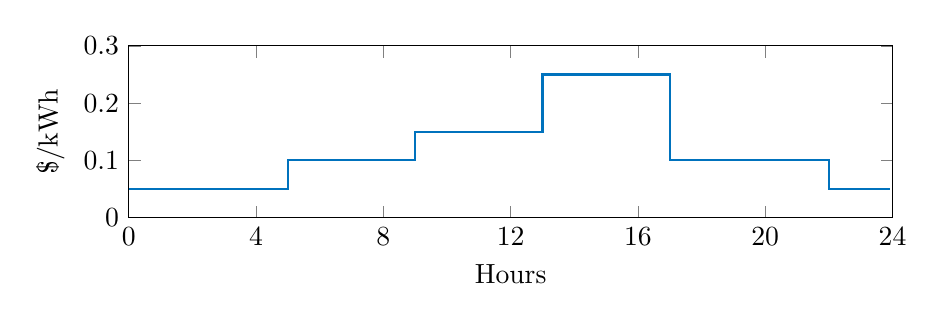
\begin{tikzpicture}
\begin{axis}[%
width=0.8\columnwidth,
height=0.18\columnwidth,
at={(1.433611in,0.649306in)},
scale only axis,
xmin=0,
xmax=24,
xlabel={Hours},
xtick={0,4,...,24},
ymin=0,
ymax=0.3,
ylabel={\$/kWh} %{Price (\$/kWh)}
]
\addplot[const plot,color=mycolor1,solid,thick] plot table[row sep=crcr] {%
0	0.05\\
0.0833333333333333	0.05\\
0.166666666666667	0.05\\
0.25	0.05\\
0.333333333333333	0.05\\
0.416666666666667	0.05\\
0.5	0.05\\
0.583333333333333	0.05\\
0.666666666666667	0.05\\
0.75	0.05\\
0.833333333333333	0.05\\
0.916666666666667	0.05\\
1	0.05\\
1.08333333333333	0.05\\
1.16666666666667	0.05\\
1.25	0.05\\
1.33333333333333	0.05\\
1.41666666666667	0.05\\
1.5	0.05\\
1.58333333333333	0.05\\
1.66666666666667	0.05\\
1.75	0.05\\
1.83333333333333	0.05\\
1.91666666666667	0.05\\
2	0.05\\
2.08333333333333	0.05\\
2.16666666666667	0.05\\
2.25	0.05\\
2.33333333333333	0.05\\
2.41666666666667	0.05\\
2.5	0.05\\
2.58333333333333	0.05\\
2.66666666666667	0.05\\
2.75	0.05\\
2.83333333333333	0.05\\
2.91666666666667	0.05\\
3	0.05\\
3.08333333333333	0.05\\
3.16666666666667	0.05\\
3.25	0.05\\
3.33333333333333	0.05\\
3.41666666666667	0.05\\
3.5	0.05\\
3.58333333333333	0.05\\
3.66666666666667	0.05\\
3.75	0.05\\
3.83333333333333	0.05\\
3.91666666666667	0.05\\
4	0.05\\
4.08333333333333	0.05\\
4.16666666666667	0.05\\
4.25	0.05\\
4.33333333333333	0.05\\
4.41666666666667	0.05\\
4.5	0.05\\
4.58333333333333	0.05\\
4.66666666666667	0.05\\
4.75	0.05\\
4.83333333333333	0.05\\
4.91666666666667	0.05\\
5	0.1\\
5.08333333333333	0.1\\
5.16666666666667	0.1\\
5.25	0.1\\
5.33333333333333	0.1\\
5.41666666666667	0.1\\
5.5	0.1\\
5.58333333333333	0.1\\
5.66666666666667	0.1\\
5.75	0.1\\
5.83333333333333	0.1\\
5.91666666666667	0.1\\
6	0.1\\
6.08333333333333	0.1\\
6.16666666666667	0.1\\
6.25	0.1\\
6.33333333333333	0.1\\
6.41666666666667	0.1\\
6.5	0.1\\
6.58333333333333	0.1\\
6.66666666666667	0.1\\
6.75	0.1\\
6.83333333333333	0.1\\
6.91666666666667	0.1\\
7	0.1\\
7.08333333333333	0.1\\
7.16666666666667	0.1\\
7.25	0.1\\
7.33333333333333	0.1\\
7.41666666666667	0.1\\
7.5	0.1\\
7.58333333333333	0.1\\
7.66666666666667	0.1\\
7.75	0.1\\
7.83333333333333	0.1\\
7.91666666666667	0.1\\
8	0.1\\
8.08333333333333	0.1\\
8.16666666666667	0.1\\
8.25	0.1\\
8.33333333333333	0.1\\
8.41666666666667	0.1\\
8.5	0.1\\
8.58333333333333	0.1\\
8.66666666666667	0.1\\
8.75	0.1\\
8.83333333333333	0.1\\
8.91666666666667	0.1\\
9	0.15\\
9.08333333333333	0.15\\
9.16666666666667	0.15\\
9.25	0.15\\
9.33333333333333	0.15\\
9.41666666666667	0.15\\
9.5	0.15\\
9.58333333333333	0.15\\
9.66666666666667	0.15\\
9.75	0.15\\
9.83333333333333	0.15\\
9.91666666666667	0.15\\
10	0.15\\
10.0833333333333	0.15\\
10.1666666666667	0.15\\
10.25	0.15\\
10.3333333333333	0.15\\
10.4166666666667	0.15\\
10.5	0.15\\
10.5833333333333	0.15\\
10.6666666666667	0.15\\
10.75	0.15\\
10.8333333333333	0.15\\
10.9166666666667	0.15\\
11	0.15\\
11.0833333333333	0.15\\
11.1666666666667	0.15\\
11.25	0.15\\
11.3333333333333	0.15\\
11.4166666666667	0.15\\
11.5	0.15\\
11.5833333333333	0.15\\
11.6666666666667	0.15\\
11.75	0.15\\
11.8333333333333	0.15\\
11.9166666666667	0.15\\
12	0.15\\
12.0833333333333	0.15\\
12.1666666666667	0.15\\
12.25	0.15\\
12.3333333333333	0.15\\
12.4166666666667	0.15\\
12.5	0.15\\
12.5833333333333	0.15\\
12.6666666666667	0.15\\
12.75	0.15\\
12.8333333333333	0.15\\
12.9166666666667	0.15\\
13	0.25\\
13.0833333333333	0.25\\
13.1666666666667	0.25\\
13.25	0.25\\
13.3333333333333	0.25\\
13.4166666666667	0.25\\
13.5	0.25\\
13.5833333333333	0.25\\
13.6666666666667	0.25\\
13.75	0.25\\
13.8333333333333	0.25\\
13.9166666666667	0.25\\
14	0.25\\
14.0833333333333	0.25\\
14.1666666666667	0.25\\
14.25	0.25\\
14.3333333333333	0.25\\
14.4166666666667	0.25\\
14.5	0.25\\
14.5833333333333	0.25\\
14.6666666666667	0.25\\
14.75	0.25\\
14.8333333333333	0.25\\
14.9166666666667	0.25\\
15	0.25\\
15.0833333333333	0.25\\
15.1666666666667	0.25\\
15.25	0.25\\
15.3333333333333	0.25\\
15.4166666666667	0.25\\
15.5	0.25\\
15.5833333333333	0.25\\
15.6666666666667	0.25\\
15.75	0.25\\
15.8333333333333	0.25\\
15.9166666666667	0.25\\
16	0.25\\
16.0833333333333	0.25\\
16.1666666666667	0.25\\
16.25	0.25\\
16.3333333333333	0.25\\
16.4166666666667	0.25\\
16.5	0.25\\
16.5833333333333	0.25\\
16.6666666666667	0.25\\
16.75	0.25\\
16.8333333333333	0.25\\
16.9166666666667	0.25\\
17	0.1\\
17.0833333333333	0.1\\
17.1666666666667	0.1\\
17.25	0.1\\
17.3333333333333	0.1\\
17.4166666666667	0.1\\
17.5	0.1\\
17.5833333333333	0.1\\
17.6666666666667	0.1\\
17.75	0.1\\
17.8333333333333	0.1\\
17.9166666666667	0.1\\
18	0.1\\
18.0833333333333	0.1\\
18.1666666666667	0.1\\
18.25	0.1\\
18.3333333333333	0.1\\
18.4166666666667	0.1\\
18.5	0.1\\
18.5833333333333	0.1\\
18.6666666666667	0.1\\
18.75	0.1\\
18.8333333333333	0.1\\
18.9166666666667	0.1\\
19	0.1\\
19.0833333333333	0.1\\
19.1666666666667	0.1\\
19.25	0.1\\
19.3333333333333	0.1\\
19.4166666666667	0.1\\
19.5	0.1\\
19.5833333333333	0.1\\
19.6666666666667	0.1\\
19.75	0.1\\
19.8333333333333	0.1\\
19.9166666666667	0.1\\
20	0.1\\
20.0833333333333	0.1\\
20.1666666666667	0.1\\
20.25	0.1\\
20.3333333333333	0.1\\
20.4166666666667	0.1\\
20.5	0.1\\
20.5833333333333	0.1\\
20.6666666666667	0.1\\
20.75	0.1\\
20.8333333333333	0.1\\
20.9166666666667	0.1\\
21	0.1\\
21.0833333333333	0.1\\
21.1666666666667	0.1\\
21.25	0.1\\
21.3333333333333	0.1\\
21.4166666666667	0.1\\
21.5	0.1\\
21.5833333333333	0.1\\
21.6666666666667	0.1\\
21.75	0.1\\
21.8333333333333	0.1\\
21.9166666666667	0.1\\
22	0.05\\
22.0833333333333	0.05\\
22.1666666666667	0.05\\
22.25	0.05\\
22.3333333333333	0.05\\
22.4166666666667	0.05\\
22.5	0.05\\
22.5833333333333	0.05\\
22.6666666666667	0.05\\
22.75	0.05\\
22.8333333333333	0.05\\
22.9166666666667	0.05\\
23	0.05\\
23.0833333333333	0.05\\
23.1666666666667	0.05\\
23.25	0.05\\
23.3333333333333	0.05\\
23.4166666666667	0.05\\
23.5	0.05\\
23.5833333333333	0.05\\
23.6666666666667	0.05\\
23.75	0.05\\
23.8333333333333	0.05\\
23.9166666666667	0.05\\
};
\end{axis}
\end{tikzpicture}%
  \caption{Time-varying price for energy demand.}
  \label{fig:simulation:price}
\end{figure}


\subsection{Complexity of the MILP} %~\protect\eqref{eq:MILP}}
\label{sec:simulation:milp}

We first tried solving the MILP~\eqref{eq:MILP} for a trivially small scale system of only two rooms ($n=m=2$) with a horizon of $N=288$ (24 hours with 5-minute sampling time), on an 8-core MacPro with 64Gb RAM running the state-of-the-art commercial solver Gurobi 6.0.
The MILP optimization did not finish after the time limit of 30 minutes and was interrupted.
Although there exist techniques to improve the performance of the optimization, for example move-blocking and warm-start, we believe that it would not scale beyond a very small number of subsystems running in real-time on a control computer with limited processing power.

\subsection{Scalable Scheduling Design}
\label{sec:simulation:design}

We performed the design process outlined in \cref{sec:summary:design} for this case study and computed the parameters of the model abstraction.
Taking the most time was the construction of the set $\Omega$ on a grid of $50 \times 50 = 2\comma 500$ cells.
Reported in red color in \cref{fig:simulation:omega} is the union of the cells resulting from this computation, for $\gamma = 20$.
To simplify $\Omega$, we took the blue polyhedron inside this union as $\Omega$.

\begin{figure}[tb]
  \centering
  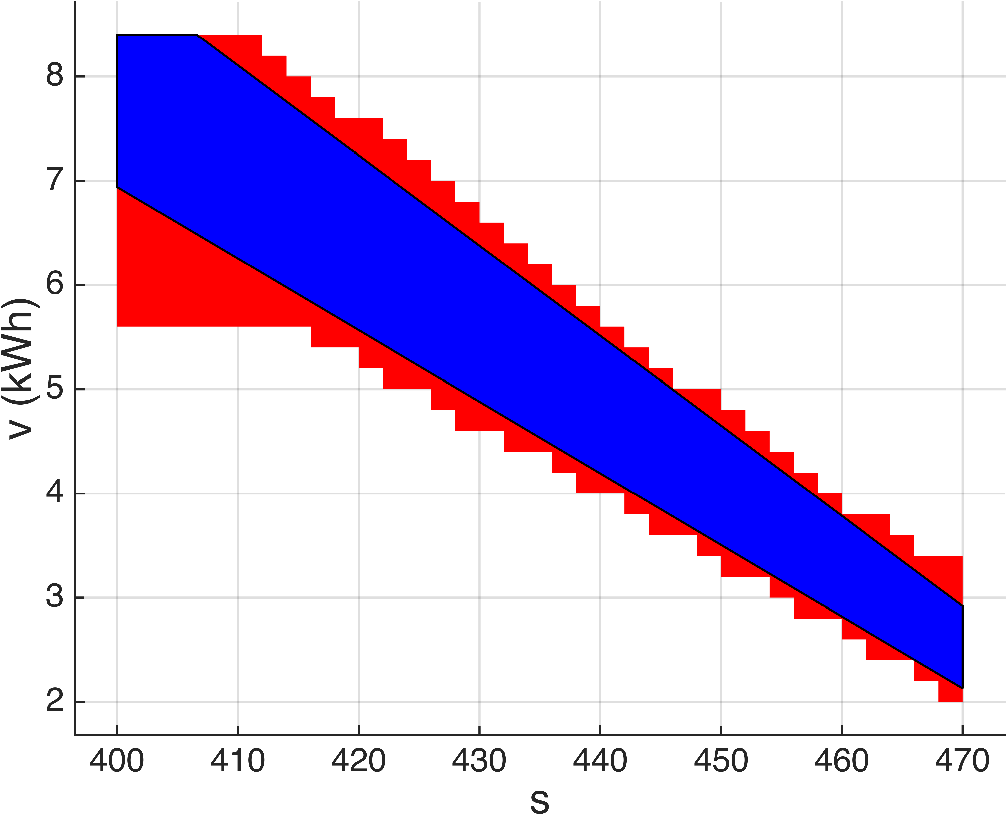
\includegraphics[width=0.8\columnwidth]{omega}
  \caption{Set $\Omega$ constructed by gridding $s$ and $v$.}
  \label{fig:simulation:omega}
\end{figure}


\subsection{Simulation Results}
\label{sec:simulation:results}

The ambient air temperature profile for 24 hours is plotted in \cref{fig:simulation:ambient}.
The internal heat gain profiles were generated following a typical pattern in office buildings.
The disturbance forecasts were generated from the actual profiles with random errors within the given accuracies.
We simulated the run-time implementation of our scheduling approach (~\cref{sec:summary:implementation}) in Matlab with Gurobi 6.0 as the optimization solver.
Each of the top-level and middle-level optimization problems took less than 15ms to be solved.
Each iteration of our scheduling algorithm took less than 30ms.
Therefore the run-time scheduling algorithm is very scalable compared to the MILP approach.

\begin{figure}[tb]
  \centering
  % This file was created by matlab2tikz.
% Minimal pgfplots version: 1.3
%
%The latest updates can be retrieved from
%  http://www.mathworks.com/matlabcentral/fileexchange/22022-matlab2tikz
%where you can also make suggestions and rate matlab2tikz.
%
\definecolor{mycolor1}{rgb}{0.00000,0.44700,0.74100}%
%
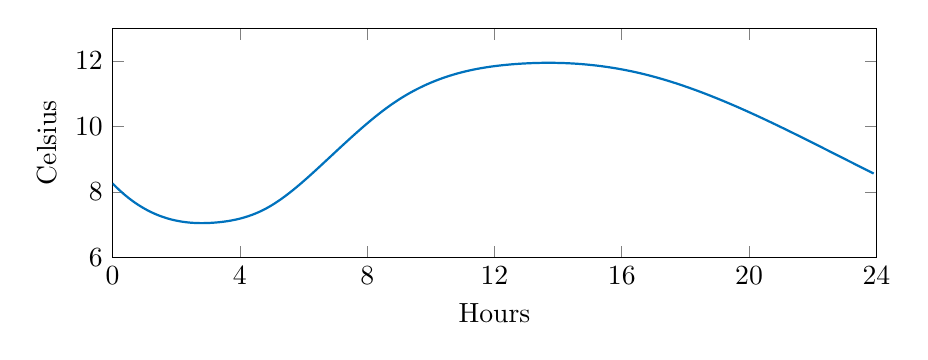
\begin{tikzpicture}

\begin{axis}[%
width=0.8\columnwidth,
height=0.24\columnwidth,
at={(1.709861in,0.710417in)},
scale only axis,
xmin=0,
xmax=24,
xlabel={Hours},
xtick={0,4,...,24},
ymin=6,
ymax=13,
ylabel={Celsius} %Temperature (C)}
]
\addplot [color=mycolor1,solid,thick,forget plot]
  table[row sep=crcr]{%
0	8.259\\
0.0833333333333333	8.17697384540428\\
0.166666666666667	8.09841840901429\\
0.25	8.0232716963163\\
0.333333333333333	7.95147171279655\\
0.416666666666667	7.88295646394131\\
0.5	7.81766395523681\\
0.583333333333333	7.75553219216933\\
0.666666666666667	7.6964991802251\\
0.75	7.6405029248904\\
0.833333333333333	7.58748143165147\\
0.916666666666667	7.53737270599456\\
1	7.49011475340593\\
1.08333333333333	7.44564557937184\\
1.16666666666667	7.40390318937854\\
1.25	7.36482558891228\\
1.33333333333333	7.32835078345932\\
1.41666666666667	7.29441677850591\\
1.5	7.26296157953831\\
1.58333333333333	7.23392319204277\\
1.66666666666667	7.20723962150555\\
1.75	7.1828488734129\\
1.83333333333333	7.16068895325107\\
1.91666666666667	7.14069786650632\\
2	7.1228136186649\\
2.08333333333333	7.10697421521307\\
2.16666666666667	7.09311766163708\\
2.25	7.08118196342319\\
2.33333333333333	7.07110512605765\\
2.41666666666667	7.06282515502672\\
2.5	7.05628005581664\\
2.58333333333333	7.05140783391368\\
2.66666666666667	7.04814649480409\\
2.75	7.04643404397412\\
2.83333333333333	7.04620848691002\\
2.91666666666667	7.04740782909806\\
3	7.04997007602449\\
3.08333333333333	7.05383323317555\\
3.16666666666667	7.05893530603751\\
3.25	7.06521444267298\\
3.33333333333333	7.07264838845224\\
3.41666666666667	7.08130835292706\\
3.5	7.09127902508022\\
3.58333333333333	7.10264509389449\\
3.66666666666667	7.11549124835265\\
3.75	7.12990217743749\\
3.83333333333333	7.14596257013177\\
3.91666666666667	7.16375711541829\\
4	7.18337050227981\\
4.08333333333333	7.20488741969912\\
4.16666666666667	7.22839255665899\\
4.25	7.25397060214221\\
4.33333333333333	7.28170624513155\\
4.41666666666667	7.3116841746098\\
4.5	7.34398907955972\\
4.58333333333333	7.37870564896411\\
4.66666666666667	7.41591857180573\\
4.75	7.45571253706737\\
4.83333333333333	7.4981722337318\\
4.91666666666667	7.54335421147295\\
5	7.59117841071421\\
5.08333333333333	7.64152337453707\\
5.16666666666667	7.69426763684603\\
5.25	7.74928973154558\\
5.33333333333333	7.80646819254021\\
5.41666666666667	7.86568155373441\\
5.5	7.92680834903268\\
5.58333333333333	7.98972711233951\\
5.66666666666667	8.0543163775594\\
5.75	8.12045467859683\\
5.83333333333333	8.1880205493563\\
5.91666666666667	8.25689252374231\\
6	8.32694913565934\\
6.08333333333333	8.39806891901188\\
6.16666666666667	8.47013040770444\\
6.25	8.54301213564151\\
6.33333333333333	8.61659263672757\\
6.41666666666667	8.69075044486713\\
6.5	8.76536409396466\\
6.58333333333333	8.84031251851373\\
6.66666666666667	8.91549412907075\\
6.75	8.99083515907236\\
6.83333333333333	9.06626397876699\\
6.91666666666667	9.14170895840307\\
7	9.21709846822903\\
7.08333333333333	9.2923608784933\\
7.16666666666667	9.36742455944431\\
7.25	9.44221788133049\\
7.33333333333333	9.51666921440026\\
7.41666666666667	9.59070692890206\\
7.5	9.66425939508431\\
7.58333333333333	9.73725498319545\\
7.66666666666667	9.80962206348391\\
7.75	9.8812890061981\\
7.83333333333333	9.95218418158647\\
7.91666666666667	10.0222359598974\\
8	10.0913727113794\\
8.08333333333333	10.1595228062809\\
8.16666666666667	10.2266146148502\\
8.25	10.2925765073359\\
8.33333333333333	10.3573368539863\\
8.41666666666667	10.4208240250499\\
8.5	10.4829663907751\\
8.58333333333333	10.5436923214104\\
8.66666666666667	10.6029301872041\\
8.75	10.6606083584046\\
8.83333333333333	10.7166552680467\\
8.91666666666667	10.7710244772014\\
9	10.8237329733915\\
9.08333333333333	10.8748075970173\\
9.16666666666667	10.9242751884787\\
9.25	10.9721625881757\\
9.33333333333333	11.0184966365084\\
9.41666666666667	11.0633041738769\\
9.5	11.1066120406812\\
9.58333333333333	11.1484470773213\\
9.66666666666667	11.1888361241974\\
9.75	11.2278060217094\\
9.83333333333333	11.2653836102574\\
9.91666666666667	11.3015957302414\\
10	11.3364692220615\\
10.0833333333333	11.3700309261178\\
10.1666666666667	11.4023076828103\\
10.25	11.433326332539\\
10.3333333333333	11.4631137157039\\
10.4166666666667	11.4916966727053\\
10.5	11.519102043943\\
10.5833333333333	11.5453566698171\\
10.6666666666667	11.5704873907277\\
10.75	11.5945210470749\\
10.8333333333333	11.6174844792586\\
10.9166666666667	11.6394045276789\\
11	11.6603080327359\\
11.0833333333333	11.6802218348297\\
11.1666666666667	11.6991727743602\\
11.25	11.7171876917275\\
11.3333333333333	11.7342934273317\\
11.4166666666667	11.7505168215728\\
11.5	11.7658847148509\\
11.5833333333333	11.780423947566\\
11.6666666666667	11.7941613601182\\
11.75	11.8071237929074\\
11.8333333333333	11.8193380863338\\
11.9166666666667	11.8308310807974\\
12	11.8416296166983\\
12.0833333333333	11.8517605344365\\
12.1666666666667	11.861250674412\\
12.25	11.8701268770249\\
12.3333333333333	11.8784159826753\\
12.4166666666667	11.8861448317631\\
12.5	11.8933402646886\\
12.5833333333333	11.9000291218515\\
12.6666666666667	11.906237993808\\
12.75	11.9119817271065\\
12.8333333333333	11.9172586206763\\
12.9166666666667	11.9220657273288\\
13	11.9264000998754\\
13.0833333333333	11.9302587911274\\
13.1666666666667	11.9336388538962\\
13.25	11.9365373409931\\
13.3333333333333	11.9389513052296\\
13.4166666666667	11.940877799417\\
13.5	11.9423138763667\\
13.5833333333333	11.9432565888901\\
13.6666666666667	11.9437029897984\\
13.75	11.9436501319032\\
13.8333333333333	11.9430950680157\\
13.9166666666667	11.9420348509473\\
14	11.9404665335095\\
14.0833333333333	11.9383871685135\\
14.1666666666667	11.9357938087708\\
14.25	11.9326835070927\\
14.3333333333333	11.9290533162906\\
14.4166666666667	11.9249002891758\\
14.5	11.9202214785597\\
14.5833333333333	11.9150139372538\\
14.6666666666667	11.9092747180693\\
14.75	11.9030008738177\\
14.8333333333333	11.8961894573102\\
14.9166666666667	11.8888375213583\\
15	11.8809421187734\\
15.0833333333333	11.8725003023668\\
15.1666666666667	11.8635091249499\\
15.25	11.8539656393341\\
15.3333333333333	11.8438668983306\\
15.4166666666667	11.833209954751\\
15.5	11.8219918614065\\
15.5833333333333	11.8102096711086\\
15.6666666666667	11.7978604366686\\
15.75	11.7849412108979\\
15.8333333333333	11.7714490466078\\
15.9166666666667	11.7573809966098\\
16	11.7427341137151\\
16.0833333333333	11.7275054507352\\
16.1666666666667	11.7116920604814\\
16.25	11.6952909957652\\
16.3333333333333	11.6782993093978\\
16.4166666666667	11.6607140541906\\
16.5	11.6425322829551\\
16.5833333333333	11.6237524587014\\
16.6666666666667	11.6043802828916\\
16.75	11.5844237730782\\
16.8333333333333	11.5638909478511\\
16.9166666666667	11.5427898258003\\
17	11.5211284255156\\
17.0833333333333	11.4989147655869\\
17.1666666666667	11.4761568646043\\
17.25	11.4528627411577\\
17.3333333333333	11.4290404138369\\
17.4166666666667	11.4046979012319\\
17.5	11.3798432219326\\
17.5833333333333	11.354484394529\\
17.6666666666667	11.328629437611\\
17.75	11.3022863697685\\
17.8333333333333	11.2754632095914\\
17.9166666666667	11.2481679756697\\
18	11.2204086865932\\
18.0833333333333	11.192193360952\\
18.1666666666667	11.163530017336\\
18.25	11.134426674335\\
18.3333333333333	11.104891350539\\
18.4166666666667	11.0749320645379\\
18.5	11.0445568349217\\
18.5833333333333	11.0137736802803\\
18.6666666666667	10.9825906192036\\
18.75	10.9510156702816\\
18.8333333333333	10.9190568521041\\
18.9166666666667	10.8867221832611\\
19	10.8540196823426\\
19.0833333333333	10.8209573679384\\
19.1666666666667	10.7875432586385\\
19.25	10.7537853730328\\
19.3333333333333	10.7196917297112\\
19.4166666666667	10.6852703472637\\
19.5	10.6505292442802\\
19.5833333333333	10.6154764393506\\
19.6666666666667	10.5801199510649\\
19.75	10.5444677980129\\
19.8333333333333	10.5085279987846\\
19.9166666666667	10.47230857197\\
20	10.435817536159\\
20.0833333333333	10.3990629099414\\
20.1666666666667	10.3620527119072\\
20.25	10.3247949606464\\
20.3333333333333	10.2872976747488\\
20.4166666666667	10.2495688728045\\
20.5	10.2116165734033\\
20.5833333333333	10.1734487951351\\
20.6666666666667	10.1350735565899\\
20.75	10.0964988763577\\
20.8333333333333	10.0577327730282\\
20.9166666666667	10.0187832651916\\
21	9.97965837143759\\
21.0833333333333	9.94036611035623\\
21.1666666666667	9.90091450053743\\
21.25	9.86131156057111\\
21.3333333333333	9.82156530904719\\
21.4166666666667	9.78168376455561\\
21.5	9.74167494568628\\
21.5833333333333	9.70154687102915\\
21.6666666666667	9.66130755917413\\
21.75	9.62096502871115\\
21.8333333333333	9.58052729823015\\
21.9166666666667	9.54000238632105\\
22	9.49939831157378\\
22.0833333333333	9.45872309257826\\
22.1666666666667	9.41798474792443\\
22.25	9.37719129620221\\
22.3333333333333	9.33635075600153\\
22.4166666666667	9.29547114591231\\
22.5	9.25456048452449\\
22.5833333333333	9.21362679042799\\
22.6666666666667	9.17267808221274\\
22.75	9.13172237846868\\
22.8333333333333	9.09076769778572\\
22.9166666666667	9.04982205875379\\
23	9.00889347996282\\
23.0833333333333	8.96798998000275\\
23.1666666666667	8.92711957746349\\
23.25	8.88629029093498\\
23.3333333333333	8.84551013900714\\
23.4166666666667	8.8047871402699\\
23.5	8.76412931331319\\
23.5833333333333	8.72354467672694\\
23.6666666666667	8.68304124910107\\
23.75	8.64262704902551\\
23.8333333333333	8.6023100950902\\
23.9166666666667	8.56209840588505\\
};
\end{axis}
\end{tikzpicture}%
  \caption{Ambient air temperature profile.}
  \label{fig:simulation:ambient}
\end{figure}

\Cref{fig:simulation:demand} plots the aggregated energy demand upper-bounds $v_{k}$ (red, dashed), computed by the top-level optimization, and the actual total energy demand $E_{k}$ (blue, solid).
Obviously, the actual aggregated energy demand $E_{k}$ never exceeded the upper-bounds $v_{k}$ set by the top-level optimization.
Also observe that the total demands, both the upper-bounds and the actual values, were lowered during the on-peak hours to reduce the cost.
The total cost for energy, including the usage charge and the peak demand charge, was $\$218.60$ with $1004.38$ kWh of consumption and $54.815$ kW peak demand.
About half of the total cost was due to the peak demand charge.

\begin{figure}[tb]
  \centering
  % This file was created by matlab2tikz.
% Minimal pgfplots version: 1.3
%
%The latest updates can be retrieved from
%  http://www.mathworks.com/matlabcentral/fileexchange/22022-matlab2tikz
%where you can also make suggestions and rate matlab2tikz.
%
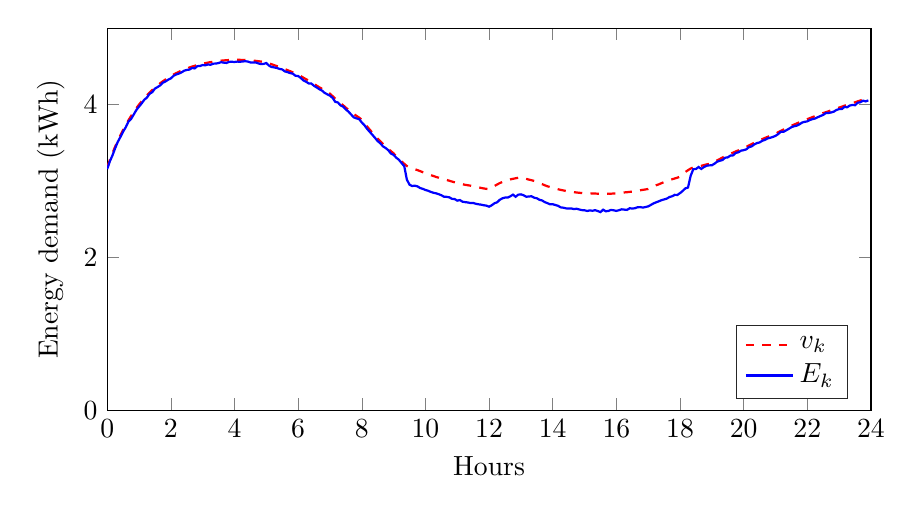
\begin{tikzpicture}

\begin{axis}[%
width=0.8\columnwidth,
height=0.4\columnwidth,
at={(1.709861in,0.710417in)},
scale only axis,
xmin=0,
xmax=24,
xlabel={Hours},
ymin=0,
ymax=5,
ylabel={Energy demand (kWh)},
legend style={at={(0.97,0.03)},anchor=south east,legend cell align=left,align=left,draw=white!15!black}
]
\addplot [color=red,dashed,thick]
  table[row sep=crcr]{%
0	3.17906616408712\\
0.0833333333333333	3.27544378698458\\
0.166666666666667	3.36493342560571\\
0.25	3.44931191986801\\
0.333333333333333	3.52769463832579\\
0.416666666666667	3.60032217763768\\
0.5	3.66893081947665\\
0.583333333333333	3.73305922231398\\
0.666666666666667	3.79394520606243\\
0.75	3.84965172680206\\
0.833333333333333	3.90361712946049\\
0.916666666666667	3.95346727260507\\
1	3.99957198393741\\
1.08333333333333	4.04325496220703\\
1.16666666666667	4.08439957734734\\
1.25	4.12213610923534\\
1.33333333333333	4.15847879388072\\
1.41666666666667	4.19108460530931\\
1.5	4.22281125340331\\
1.58333333333333	4.25130392182489\\
1.66666666666667	4.27933114524643\\
1.75	4.30540750459767\\
1.83333333333333	4.32907055426529\\
1.91666666666667	4.3519134038166\\
2	4.37347012839873\\
2.08333333333333	4.39393385481135\\
2.16666666666667	4.41175500494223\\
2.25	4.42848339127525\\
2.33333333333333	4.4445686780251\\
2.41666666666667	4.45955567293209\\
2.5	4.47287023263901\\
2.58333333333333	4.48546938228343\\
2.66666666666667	4.49751075305313\\
2.75	4.50805271150403\\
2.83333333333333	4.51879299045348\\
2.91666666666667	4.5274002322555\\
3	4.53574988704158\\
3.08333333333333	4.54295104730042\\
3.16666666666667	4.54999378781973\\
3.25	4.55607346042376\\
3.33333333333333	4.56235262915517\\
3.41666666666667	4.56739294034205\\
3.5	4.57176446352992\\
3.58333333333333	4.57560328835473\\
3.66666666666667	4.57843502535881\\
3.75	4.5812721203605\\
3.83333333333333	4.58391101458455\\
3.91666666666667	4.58495481302594\\
4	4.58564876320178\\
4.08333333333333	4.58621753821269\\
4.16666666666667	4.58606561123249\\
4.25	4.58517282853045\\
4.33333333333333	4.58368693832529\\
4.41666666666667	4.58135288446176\\
4.5	4.57863355560453\\
4.58333333333333	4.57574807180291\\
4.66666666666667	4.572594053468\\
4.75	4.56827150188052\\
4.83333333333333	4.56397683049059\\
4.91666666666667	4.55934769899874\\
5	4.55361236477936\\
5.08333333333333	4.54011153951938\\
5.16666666666667	4.52813196314243\\
5.25	4.51613896726423\\
5.33333333333333	4.50391457834235\\
5.41666666666667	4.49090851411491\\
5.5	4.47770303563728\\
5.58333333333333	4.46405803734461\\
5.66666666666667	4.45073298377598\\
5.75	4.43728990819075\\
5.83333333333333	4.42304881780525\\
5.91666666666667	4.40836129546487\\
6	4.39400445422722\\
6.08333333333333	4.37237701641462\\
6.16666666666667	4.35203099181993\\
6.25	4.33221404408187\\
6.33333333333333	4.31267441606578\\
6.41666666666667	4.29339456734824\\
6.5	4.27162908064057\\
6.58333333333333	4.24761175177522\\
6.66666666666667	4.22617557241438\\
6.75	4.2072705422975\\
6.83333333333333	4.18662501967539\\
6.91666666666667	4.16362029931698\\
7	4.14331914257393\\
7.08333333333333	4.11045224247844\\
7.16666666666667	4.0771826222038\\
7.25	4.04817186231294\\
7.33333333333333	4.01721211340898\\
7.41666666666667	3.98970620492086\\
7.5	3.95977843797079\\
7.58333333333333	3.93018283570909\\
7.66666666666667	3.90046764186681\\
7.75	3.874980611039\\
7.83333333333333	3.85313092988834\\
7.91666666666667	3.82889570334821\\
8	3.8037196881149\\
8.08333333333333	3.75672844792987\\
8.16666666666667	3.71255378791877\\
8.25	3.67208686852458\\
8.33333333333333	3.63184591181729\\
8.41666666666667	3.59190509904319\\
8.5	3.55268447587664\\
8.58333333333333	3.51904197107396\\
8.66666666666667	3.48403248266199\\
8.75	3.45296080386042\\
8.83333333333333	3.42083026828082\\
8.91666666666667	3.39013080797302\\
9	3.36099447425266\\
9.08333333333333	3.32493662604052\\
9.16666666666667	3.29021548441556\\
9.25	3.25558464125971\\
9.33333333333333	3.22510685804794\\
9.41666666666667	3.19550497613841\\
9.5	3.17879356897274\\
9.58333333333333	3.16485189944042\\
9.66666666666667	3.15331672507216\\
9.75	3.14195278004129\\
9.83333333333333	3.12920354304148\\
9.91666666666667	3.11493556206932\\
10	3.10197456661298\\
10.0833333333333	3.08907934526332\\
10.1666666666667	3.07700755656166\\
10.25	3.06540281871519\\
10.3333333333333	3.05276592838011\\
10.4166666666667	3.04257485296102\\
10.5	3.0302054337391\\
10.5833333333333	3.02186285143193\\
10.6666666666667	3.01359068542177\\
10.75	3.00306122911023\\
10.8333333333333	2.9924979299991\\
10.9166666666667	2.98296527521139\\
11	2.97445065082732\\
11.0833333333333	2.96710260297565\\
11.1666666666667	2.95765564003974\\
11.25	2.94960457284546\\
11.3333333333333	2.94390867450586\\
11.4166666666667	2.93846098424384\\
11.5	2.93061963907972\\
11.5833333333333	2.92257087268562\\
11.6666666666667	2.91577768739161\\
11.75	2.90908914629377\\
11.8333333333333	2.90193817973302\\
11.9166666666667	2.89700620810567\\
12	2.89212971776521\\
12.0833333333333	2.91405990912183\\
12.1666666666667	2.93360474419576\\
12.25	2.95345575444909\\
12.3333333333333	2.97191143039134\\
12.4166666666667	2.98686845379345\\
12.5	3.00219618718543\\
12.5833333333333	3.01054525714215\\
12.6666666666667	3.02087140951809\\
12.75	3.02849646429365\\
12.8333333333333	3.03552323739019\\
12.9166666666667	3.04257975323383\\
13	3.04882938626437\\
13.0833333333333	3.03697342748501\\
13.1666666666667	3.02802202545447\\
13.25	3.01805588019655\\
13.3333333333333	3.01021929489416\\
13.4166666666667	3.00018925190345\\
13.5	2.98889675662506\\
13.5833333333333	2.97238582874171\\
13.6666666666667	2.95891598276798\\
13.75	2.94365825716788\\
13.8333333333333	2.93062592510692\\
13.9166666666667	2.92069655476621\\
14	2.91084949790844\\
14.0833333333333	2.90104265178913\\
14.1666666666667	2.89208373867565\\
14.25	2.88334013131991\\
14.3333333333333	2.87628693825762\\
14.4166666666667	2.8690966820319\\
14.5	2.86297138383291\\
14.5833333333333	2.85933731354203\\
14.6666666666667	2.85341117400293\\
14.75	2.84915280255638\\
14.8333333333333	2.84564577667663\\
14.9166666666667	2.84193095193359\\
15	2.83839078079379\\
15.0833333333333	2.83700569369891\\
15.1666666666667	2.83539206913733\\
15.25	2.83654193670316\\
15.3333333333333	2.83511174717724\\
15.4166666666667	2.83368045018795\\
15.5	2.83228959053585\\
15.5833333333333	2.83447536043477\\
15.6666666666667	2.83337107417398\\
15.75	2.83422573522877\\
15.8333333333333	2.83401061459356\\
15.9166666666667	2.83524609215136\\
16	2.83599676549821\\
16.0833333333333	2.83962079651645\\
16.1666666666667	2.84505061429937\\
16.25	2.85004157334932\\
16.3333333333333	2.85306377160763\\
16.4166666666667	2.85738642025137\\
16.5	2.86044941109602\\
16.5833333333333	2.866748349852\\
16.6666666666667	2.87331372290892\\
16.75	2.87810429853608\\
16.8333333333333	2.88399629855069\\
16.9166666666667	2.88937194463174\\
17	2.89533426803884\\
17.0833333333333	2.91326058802615\\
17.1666666666667	2.92829706284216\\
17.25	2.94404334058894\\
17.3333333333333	2.9561664840812\\
17.4166666666667	2.97142960879255\\
17.5	2.98526563277654\\
17.5833333333333	2.9993075540124\\
17.6666666666667	3.0113417282933\\
17.75	3.02246800256442\\
17.8333333333333	3.03290397991592\\
17.9166666666667	3.04320010466643\\
18	3.0568921624554\\
18.0833333333333	3.08643980310983\\
18.1666666666667	3.11700664235435\\
18.25	3.14139617930249\\
18.3333333333333	3.16284440760376\\
18.4166666666667	3.17723589312949\\
18.5	3.182078068803\\
18.5833333333333	3.18894857512526\\
18.6666666666667	3.19823969656732\\
18.75	3.20796215314075\\
18.8333333333333	3.21718474691731\\
18.9166666666667	3.22429782525796\\
19	3.23018355547638\\
19.0833333333333	3.25030474051133\\
19.1666666666667	3.2699556813687\\
19.25	3.28820429772806\\
19.3333333333333	3.30630618498787\\
19.4166666666667	3.32413634788268\\
19.5	3.34027240067061\\
19.5833333333333	3.35640077606773\\
19.6666666666667	3.37133406236698\\
19.75	3.38707329735521\\
19.8333333333333	3.40078143431299\\
19.9166666666667	3.41417267151753\\
20	3.42750302554169\\
20.0833333333333	3.44681014009008\\
20.1666666666667	3.46588417090195\\
20.25	3.48319123473082\\
20.3333333333333	3.50097413938048\\
20.4166666666667	3.51698060239412\\
20.5	3.53248352620674\\
20.5833333333333	3.54842779711344\\
20.6666666666667	3.56311880361411\\
20.75	3.57755629378072\\
20.8333333333333	3.59119303613569\\
20.9166666666667	3.60512849896216\\
21	3.61905992486094\\
21.0833333333333	3.6381765611166\\
21.1666666666667	3.65649587006742\\
21.25	3.67288114399418\\
21.3333333333333	3.69031705168413\\
21.4166666666667	3.70677914759907\\
21.5	3.72292232175547\\
21.5833333333333	3.73833554234034\\
21.6666666666667	3.75316317954729\\
21.75	3.76819820600529\\
21.8333333333333	3.78287405234077\\
21.9166666666667	3.7961775657245\\
22	3.80980572992141\\
22.0833333333333	3.82358538443084\\
22.1666666666667	3.83691555150421\\
22.25	3.8501206798408\\
22.3333333333333	3.86354503476749\\
22.4166666666667	3.87677026478994\\
22.5	3.88923165078782\\
22.5833333333333	3.90152443585214\\
22.6666666666667	3.91313398510924\\
22.75	3.92512059402401\\
22.8333333333333	3.93738280341439\\
22.9166666666667	3.94962047616778\\
23	3.96089584461422\\
23.0833333333333	3.97269850128404\\
23.1666666666667	3.98518527521872\\
23.25	3.99592732633446\\
23.3333333333333	4.00774254337837\\
23.4166666666667	4.01911329735522\\
23.5	4.0304099116611\\
23.5833333333333	4.04278263911675\\
23.6666666666667	4.05371192845171\\
23.75	4.06525298992051\\
23.8333333333333	4.07582410479744\\
23.9166666666667	4.08798290785191\\
};
\addlegendentry{$v_{k}$};

\addplot [color=blue,solid,thick]
  table[row sep=crcr]{%
0	3.155\\
0.0833333333333333	3.25666666666667\\
0.166666666666667	3.33625\\
0.25	3.42833333333333\\
0.333333333333333	3.5125\\
0.416666666666667	3.57666666666667\\
0.5	3.64625\\
0.583333333333333	3.70333333333333\\
0.666666666666667	3.77666666666667\\
0.75	3.81166666666667\\
0.833333333333333	3.86958333333333\\
0.916666666666667	3.92958333333333\\
1	3.97333333333333\\
1.08333333333333	4.01625\\
1.16666666666667	4.06375\\
1.25	4.09291666666667\\
1.33333333333333	4.14208333333333\\
1.41666666666667	4.16291666666667\\
1.5	4.20958333333333\\
1.58333333333333	4.22958333333333\\
1.66666666666667	4.25208333333333\\
1.75	4.28708333333333\\
1.83333333333333	4.30291666666667\\
1.91666666666667	4.32666666666667\\
2	4.34291666666667\\
2.08333333333333	4.37583333333333\\
2.16666666666667	4.39375\\
2.25	4.40541666666667\\
2.33333333333333	4.42125\\
2.41666666666667	4.44333333333333\\
2.5	4.45375\\
2.58333333333333	4.45833333333333\\
2.66666666666667	4.47958333333333\\
2.75	4.47416666666667\\
2.83333333333333	4.50333333333333\\
2.91666666666667	4.50541666666667\\
3	4.5175\\
3.08333333333333	4.515\\
3.16666666666667	4.52458333333333\\
3.25	4.52208333333333\\
3.33333333333333	4.53583333333333\\
3.41666666666667	4.5375\\
3.5	4.54416666666667\\
3.58333333333333	4.55541666666667\\
3.66666666666667	4.54875\\
3.75	4.54583333333333\\
3.83333333333333	4.55958333333333\\
3.91666666666667	4.56083333333333\\
4	4.55791666666667\\
4.08333333333333	4.56291666666667\\
4.16666666666667	4.56083333333333\\
4.25	4.56416666666667\\
4.33333333333333	4.56791666666667\\
4.41666666666667	4.56416666666667\\
4.5	4.55208333333333\\
4.58333333333333	4.55\\
4.66666666666667	4.5525\\
4.75	4.53958333333333\\
4.83333333333333	4.53041666666667\\
4.91666666666667	4.53333333333333\\
5	4.54416666666667\\
5.08333333333333	4.51041666666667\\
5.16666666666667	4.49291666666667\\
5.25	4.48666666666667\\
5.33333333333333	4.47958333333333\\
5.41666666666667	4.46708333333333\\
5.5	4.46041666666667\\
5.58333333333333	4.43458333333333\\
5.66666666666667	4.425\\
5.75	4.4125\\
5.83333333333333	4.405\\
5.91666666666667	4.37708333333333\\
6	4.37458333333333\\
6.08333333333333	4.34791666666667\\
6.16666666666667	4.31625\\
6.25	4.29958333333333\\
6.33333333333333	4.27708333333333\\
6.41666666666667	4.27541666666667\\
6.5	4.24541666666667\\
6.58333333333333	4.22458333333333\\
6.66666666666667	4.20125\\
6.75	4.18333333333333\\
6.83333333333333	4.15333333333333\\
6.91666666666667	4.13458333333333\\
7	4.11666666666667\\
7.08333333333333	4.08791666666667\\
7.16666666666667	4.03666666666667\\
7.25	4.0275\\
7.33333333333333	3.98916666666667\\
7.41666666666667	3.9725\\
7.5	3.93541666666667\\
7.58333333333333	3.9075\\
7.66666666666667	3.86916666666667\\
7.75	3.83291666666667\\
7.83333333333333	3.81958333333333\\
7.91666666666667	3.81\\
8	3.76625\\
8.08333333333333	3.73\\
8.16666666666667	3.6825\\
8.25	3.64333333333333\\
8.33333333333333	3.60458333333333\\
8.41666666666667	3.56375\\
8.5	3.52125\\
8.58333333333333	3.49291666666667\\
8.66666666666667	3.45291666666667\\
8.75	3.43166666666667\\
8.83333333333333	3.40291666666667\\
8.91666666666667	3.35833333333333\\
9	3.34166666666667\\
9.08333333333333	3.30458333333333\\
9.16666666666667	3.27791666666667\\
9.25	3.23458333333333\\
9.33333333333333	3.195\\
9.41666666666667	3.01833333333333\\
9.5	2.95083333333333\\
9.58333333333333	2.93416666666667\\
9.66666666666667	2.93833333333333\\
9.75	2.92916666666667\\
9.83333333333333	2.9075\\
9.91666666666667	2.89708333333333\\
10	2.88208333333333\\
10.0833333333333	2.87208333333333\\
10.1666666666667	2.85708333333333\\
10.25	2.84541666666667\\
10.3333333333333	2.83833333333333\\
10.4166666666667	2.82708333333333\\
10.5	2.81333333333333\\
10.5833333333333	2.79375\\
10.6666666666667	2.79208333333333\\
10.75	2.78583333333333\\
10.8333333333333	2.76625\\
10.9166666666667	2.76333333333333\\
11	2.7425\\
11.0833333333333	2.75\\
11.1666666666667	2.72833333333333\\
11.25	2.72291666666667\\
11.3333333333333	2.71875\\
11.4166666666667	2.71041666666667\\
11.5	2.71208333333333\\
11.5833333333333	2.70166666666667\\
11.6666666666667	2.69458333333333\\
11.75	2.69\\
11.8333333333333	2.68208333333333\\
11.9166666666667	2.67708333333333\\
12	2.66333333333333\\
12.0833333333333	2.68208333333333\\
12.1666666666667	2.70791666666667\\
12.25	2.72\\
12.3333333333333	2.75333333333333\\
12.4166666666667	2.7725\\
12.5	2.7825\\
12.5833333333333	2.78291666666667\\
12.6666666666667	2.79875\\
12.75	2.82125\\
12.8333333333333	2.79333333333333\\
12.9166666666667	2.82041666666667\\
13	2.825\\
13.0833333333333	2.81291666666667\\
13.1666666666667	2.79375\\
13.25	2.79666666666667\\
13.3333333333333	2.8\\
13.4166666666667	2.78083333333333\\
13.5	2.77375\\
13.5833333333333	2.75375\\
13.6666666666667	2.74458333333333\\
13.75	2.72291666666667\\
13.8333333333333	2.71\\
13.9166666666667	2.69375\\
14	2.69625\\
14.0833333333333	2.685\\
14.1666666666667	2.675\\
14.25	2.65458333333333\\
14.3333333333333	2.65\\
14.4166666666667	2.64166666666667\\
14.5	2.63833333333333\\
14.5833333333333	2.64041666666667\\
14.6666666666667	2.63166666666667\\
14.75	2.63666666666667\\
14.8333333333333	2.62666666666667\\
14.9166666666667	2.61875\\
15	2.61625\\
15.0833333333333	2.6075\\
15.1666666666667	2.615\\
15.25	2.61\\
15.3333333333333	2.61791666666667\\
15.4166666666667	2.60625\\
15.5	2.5925\\
15.5833333333333	2.62416666666667\\
15.6666666666667	2.60291666666667\\
15.75	2.60833333333333\\
15.8333333333333	2.62125\\
15.9166666666667	2.61583333333333\\
16	2.60833333333333\\
16.0833333333333	2.6175\\
16.1666666666667	2.62916666666667\\
16.25	2.625\\
16.3333333333333	2.62125\\
16.4166666666667	2.6425\\
16.5	2.63958333333333\\
16.5833333333333	2.64291666666667\\
16.6666666666667	2.65666666666667\\
16.75	2.65791666666667\\
16.8333333333333	2.65166666666667\\
16.9166666666667	2.65916666666667\\
17	2.6675\\
17.0833333333333	2.68666666666667\\
17.1666666666667	2.70708333333333\\
17.25	2.72083333333333\\
17.3333333333333	2.73375\\
17.4166666666667	2.74875\\
17.5	2.75875\\
17.5833333333333	2.76875\\
17.6666666666667	2.79\\
17.75	2.79916666666667\\
17.8333333333333	2.81833333333333\\
17.9166666666667	2.8175\\
18	2.84125\\
18.0833333333333	2.86958333333333\\
18.1666666666667	2.90333333333333\\
18.25	2.91416666666667\\
18.3333333333333	3.06708333333333\\
18.4166666666667	3.15416666666667\\
18.5	3.15708333333333\\
18.5833333333333	3.18291666666667\\
18.6666666666667	3.15791666666667\\
18.75	3.18125\\
18.8333333333333	3.19958333333333\\
18.9166666666667	3.20416666666667\\
19	3.20583333333333\\
19.0833333333333	3.22666666666667\\
19.1666666666667	3.25291666666667\\
19.25	3.26458333333333\\
19.3333333333333	3.27458333333333\\
19.4166666666667	3.30458333333333\\
19.5	3.30875\\
19.5833333333333	3.3325\\
19.6666666666667	3.33541666666667\\
19.75	3.36708333333333\\
19.8333333333333	3.37541666666667\\
19.9166666666667	3.39708333333333\\
20	3.40333333333333\\
20.0833333333333	3.41458333333333\\
20.1666666666667	3.44416666666667\\
20.25	3.4525\\
20.3333333333333	3.47833333333333\\
20.4166666666667	3.49625\\
20.5	3.50458333333333\\
20.5833333333333	3.52625\\
20.6666666666667	3.5375\\
20.75	3.55708333333333\\
20.8333333333333	3.56583333333333\\
20.9166666666667	3.57666666666667\\
21	3.59083333333333\\
21.0833333333333	3.61416666666667\\
21.1666666666667	3.64416666666667\\
21.25	3.64291666666667\\
21.3333333333333	3.66291666666667\\
21.4166666666667	3.6825\\
21.5	3.70416666666667\\
21.5833333333333	3.71708333333333\\
21.6666666666667	3.72416666666667\\
21.75	3.74083333333333\\
21.8333333333333	3.765\\
21.9166666666667	3.77458333333333\\
22	3.78083333333333\\
22.0833333333333	3.79958333333333\\
22.1666666666667	3.81041666666667\\
22.25	3.81916666666667\\
22.3333333333333	3.83583333333333\\
22.4166666666667	3.85125\\
22.5	3.86583333333333\\
22.5833333333333	3.89\\
22.6666666666667	3.89041666666667\\
22.75	3.8975\\
22.8333333333333	3.90791666666667\\
22.9166666666667	3.93041666666667\\
23	3.94166666666667\\
23.0833333333333	3.94083333333333\\
23.1666666666667	3.97041666666667\\
23.25	3.965\\
23.3333333333333	3.9875\\
23.4166666666667	3.99541666666667\\
23.5	3.99208333333333\\
23.5833333333333	4.02416666666667\\
23.6666666666667	4.03125\\
23.75	4.05125\\
23.8333333333333	4.04208333333333\\
23.9166666666667	4.055\\
};
\addlegendentry{$E_k$};

\end{axis}
\end{tikzpicture}%
  \caption{Aggregated energy demand upper-bounds $v_{k}$ computed by the top-level optimization and the actual demands $E_{k}$.}
  \label{fig:simulation:demand}
\end{figure}


\Cref{fig:simulation:temp} reports the air temperatures for the first 4 rooms.
It can be seen that the temperatures were always maintained inside the required comfort range.

\begin{figure}[tb]
  \centering
  % This file was created by matlab2tikz.
% Minimal pgfplots version: 1.3
%
%The latest updates can be retrieved from
%  http://www.mathworks.com/matlabcentral/fileexchange/22022-matlab2tikz
%where you can also make suggestions and rate matlab2tikz.
%
\definecolor{mycolor1}{rgb}{0.00000,0.44700,0.74100}%
\definecolor{mycolor2}{rgb}{0.85000,0.32500,0.09800}%
\definecolor{mycolor3}{rgb}{0.92900,0.69400,0.12500}%
\definecolor{mycolor4}{rgb}{0.49400,0.18400,0.55600}%
%
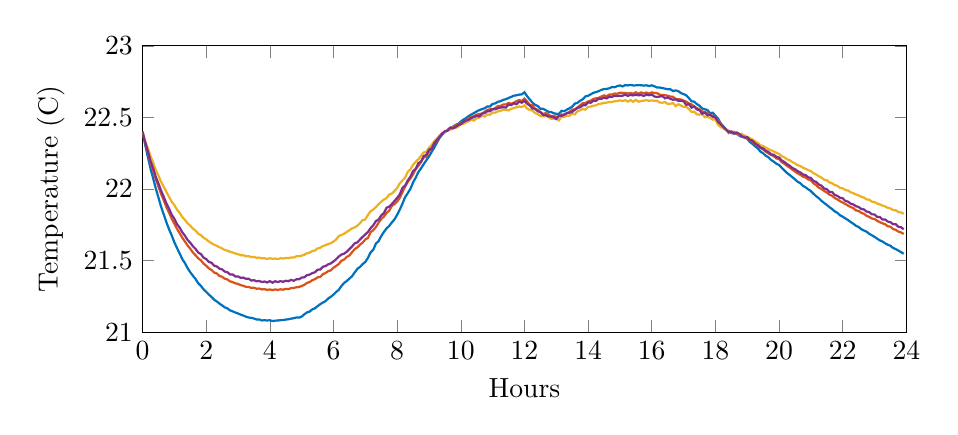
\begin{tikzpicture}

\begin{axis}[%
width=0.8\columnwidth,
height=0.3\columnwidth,
at={(1.709861in,0.710417in)},
scale only axis,
xmin=0,
xmax=24,
xlabel={Hours},
ymin=21,
ymax=23,
ylabel={Temperature (C)}
]
\addplot [color=mycolor1,solid,thick,forget plot]
  table[row sep=crcr]{%
0	22.4\\
0.0833333333333333	22.3086043458914\\
0.166666666666667	22.2242611911255\\
0.25	22.1434048533607\\
0.333333333333333	22.0741790488466\\
0.416666666666667	22.0036172465766\\
0.5	21.9402488140146\\
0.583333333333333	21.8756192248584\\
0.666666666666667	21.8220013628992\\
0.75	21.7673497470895\\
0.833333333333333	21.7188532892887\\
0.916666666666667	21.6756638655975\\
1	21.6279043886627\\
1.08333333333333	21.5878697168294\\
1.16666666666667	21.5504568317053\\
1.25	21.5104501147984\\
1.33333333333333	21.4822336556636\\
1.41666666666667	21.4472350212314\\
1.5	21.4190448572608\\
1.58333333333333	21.3944029629408\\
1.66666666666667	21.371188357887\\
1.75	21.3419491557966\\
1.83333333333333	21.3238852285944\\
1.91666666666667	21.2994127887635\\
2	21.282540819207\\
2.08333333333333	21.2629724526907\\
2.16666666666667	21.2467075233767\\
2.25	21.2272880021003\\
2.33333333333333	21.2146580405542\\
2.41666666666667	21.2002520212816\\
2.5	21.1877942145956\\
2.58333333333333	21.1736367277546\\
2.66666666666667	21.1664813582731\\
2.75	21.1525664489696\\
2.83333333333333	21.1456966001865\\
2.91666666666667	21.1376480900443\\
3	21.1310228438314\\
3.08333333333333	21.1227020258404\\
3.16666666666667	21.1164834781353\\
3.25	21.1085538971185\\
3.33333333333333	21.1027215807123\\
3.41666666666667	21.1005446884473\\
3.5	21.0961306392933\\
3.58333333333333	21.0890412283554\\
3.66666666666667	21.0891064012099\\
3.75	21.0825117151603\\
3.83333333333333	21.0834911007038\\
3.91666666666667	21.0824050536893\\
4	21.083482361918\\
4.08333333333333	21.0785218432875\\
4.16666666666667	21.0808569184993\\
4.25	21.0818380343805\\
4.33333333333333	21.084288779537\\
4.41666666666667	21.0852400012525\\
4.5	21.0885006594532\\
4.58333333333333	21.0907355062237\\
4.66666666666667	21.0949458251553\\
4.75	21.0977206101355\\
4.83333333333333	21.1030394841602\\
4.91666666666667	21.101943932494\\
5	21.109160226637\\
5.08333333333333	21.1249308796111\\
5.16666666666667	21.1384291251325\\
5.25	21.1442567353548\\
5.33333333333333	21.1597718369646\\
5.41666666666667	21.1670109495695\\
5.5	21.1822911081631\\
5.58333333333333	21.1958120070656\\
5.66666666666667	21.2075033665786\\
5.75	21.2175137325423\\
5.83333333333333	21.2353846368832\\
5.91666666666667	21.2477327870638\\
6	21.2628307303502\\
6.08333333333333	21.2813823949768\\
6.16666666666667	21.2960124942309\\
6.25	21.3229396998879\\
6.33333333333333	21.3440720716609\\
6.41666666666667	21.3581786606819\\
6.5	21.3744563208192\\
6.58333333333333	21.3911617338408\\
6.66666666666667	21.417837237158\\
6.75	21.4426456372009\\
6.83333333333333	21.4562091474116\\
6.91666666666667	21.4759750975508\\
7	21.4909570569607\\
7.08333333333333	21.5198240308517\\
7.16666666666667	21.557566833543\\
7.25	21.5758378173804\\
7.33333333333333	21.6195638470479\\
7.41666666666667	21.6357983231085\\
7.5	21.6716235834034\\
7.58333333333333	21.7002512407997\\
7.66666666666667	21.7247577840578\\
7.75	21.7422215096203\\
7.83333333333333	21.7665033131309\\
7.91666666666667	21.7877448250509\\
8	21.8205660671853\\
8.08333333333333	21.8561350139551\\
8.16666666666667	21.8975704344473\\
8.25	21.9439846635429\\
8.33333333333333	21.9709017770205\\
8.41666666666667	22.0016929601674\\
8.5	22.0456759782908\\
8.58333333333333	22.0792571765408\\
8.66666666666667	22.1184628348523\\
8.75	22.1442245430127\\
8.83333333333333	22.1737313199309\\
8.91666666666667	22.2007042292074\\
9	22.2264692053883\\
9.08333333333333	22.2589950932754\\
9.16666666666667	22.2894074284019\\
9.25	22.3246178570238\\
9.33333333333333	22.3569654430934\\
9.41666666666667	22.3804583456407\\
9.5	22.3965836198916\\
9.58333333333333	22.413242591797\\
9.66666666666667	22.4266846333268\\
9.75	22.4333923207877\\
9.83333333333333	22.4476680468469\\
9.91666666666667	22.4549669222719\\
10	22.4709606441577\\
10.0833333333333	22.4848044349149\\
10.1666666666667	22.4951635149677\\
10.25	22.5095844667474\\
10.3333333333333	22.5206158060622\\
10.4166666666667	22.5305249027215\\
10.5	22.5420807202934\\
10.5833333333333	22.5511721478954\\
10.6666666666667	22.5581444355977\\
10.75	22.5640672791326\\
10.8333333333333	22.5765941239749\\
10.9166666666667	22.5762862444606\\
11	22.5943423819239\\
11.0833333333333	22.5978433661995\\
11.1666666666667	22.6092255043755\\
11.25	22.6135500751825\\
11.3333333333333	22.6228522800448\\
11.4166666666667	22.6271583413896\\
11.5	22.6359374710506\\
11.5833333333333	22.6432335484133\\
11.6666666666667	22.6517894941846\\
11.75	22.6544840124855\\
11.8333333333333	22.6590700893572\\
11.9166666666667	22.6608929280262\\
12	22.6753648796094\\
12.0833333333333	22.6482469479472\\
12.1666666666667	22.6260867155776\\
12.25	22.6033938999291\\
12.3333333333333	22.5875809825871\\
12.4166666666667	22.5804231371114\\
12.5	22.5602062711177\\
12.5833333333333	22.5605277453782\\
12.6666666666667	22.5507856398527\\
12.75	22.5397188666618\\
12.8333333333333	22.537213140684\\
12.9166666666667	22.5302073629803\\
13	22.524798813058\\
13.0833333333333	22.5249183194283\\
13.1666666666667	22.5461698116627\\
13.25	22.543111674015\\
13.3333333333333	22.5544358728826\\
13.4166666666667	22.5636464575132\\
13.5	22.5752230176855\\
13.5833333333333	22.596362095501\\
13.6666666666667	22.6019541539423\\
13.75	22.616415456022\\
13.8333333333333	22.6266763665204\\
13.9166666666667	22.6469747067415\\
14	22.6512510737682\\
14.0833333333333	22.6611480475682\\
14.1666666666667	22.6721759279131\\
14.25	22.6766809046465\\
14.3333333333333	22.6834732910916\\
14.4166666666667	22.6926409399427\\
14.5	22.6979085530527\\
14.5833333333333	22.6991974178105\\
14.6666666666667	22.703636591565\\
14.75	22.7121683916208\\
14.8333333333333	22.7106385394122\\
14.9166666666667	22.7188379317732\\
15	22.7231130540567\\
15.0833333333333	22.7168237538818\\
15.1666666666667	22.725894266278\\
15.25	22.7233936416554\\
15.3333333333333	22.7270622567213\\
15.4166666666667	22.723298234211\\
15.5	22.7238043799788\\
15.5833333333333	22.7257131796982\\
15.6666666666667	22.7249558663779\\
15.75	22.7217918407685\\
15.8333333333333	22.7244794966043\\
15.9166666666667	22.7189799865379\\
16	22.7241569488208\\
16.0833333333333	22.7173500354316\\
16.1666666666667	22.7080200744816\\
16.25	22.7091085734196\\
16.3333333333333	22.7051728396991\\
16.4166666666667	22.7010909537034\\
16.5	22.6968911895218\\
16.5833333333333	22.6965369002885\\
16.6666666666667	22.6842198117188\\
16.75	22.688510681897\\
16.8333333333333	22.683707562433\\
16.9166666666667	22.6697662650914\\
17	22.663003779671\\
17.0833333333333	22.6546684123504\\
17.1666666666667	22.6348906543403\\
17.25	22.6131215280926\\
17.3333333333333	22.6096951262968\\
17.4166666666667	22.5931873105059\\
17.5	22.5819297871968\\
17.5833333333333	22.562833768499\\
17.6666666666667	22.5572102021859\\
17.75	22.5510529702668\\
17.8333333333333	22.5294546226832\\
17.9166666666667	22.5329528278386\\
18	22.5110125330367\\
18.0833333333333	22.491562660565\\
18.1666666666667	22.4583811767831\\
18.25	22.4371144300592\\
18.3333333333333	22.4157685765473\\
18.4166666666667	22.4052182324258\\
18.5	22.391100903358\\
18.5833333333333	22.3881777173486\\
18.6666666666667	22.38644057662\\
18.75	22.3727549079883\\
18.8333333333333	22.3645587803789\\
18.9166666666667	22.3604009498411\\
19	22.3505510289999\\
19.0833333333333	22.3288473166747\\
19.1666666666667	22.3147349687618\\
19.25	22.2979333842525\\
19.3333333333333	22.2831517489604\\
19.4166666666667	22.2608846222877\\
19.5	22.2492242627456\\
19.5833333333333	22.2323240273214\\
19.6666666666667	22.2214452489894\\
19.75	22.2026668806133\\
19.8333333333333	22.1911261127319\\
19.9166666666667	22.176425950013\\
20	22.1683019916466\\
20.0833333333333	22.1482223509744\\
20.1666666666667	22.1304606148621\\
20.25	22.1119405251311\\
20.3333333333333	22.0979825090007\\
20.4166666666667	22.082906403196\\
20.5	22.0678071776163\\
20.5833333333333	22.0512260900955\\
20.6666666666667	22.0406806984158\\
20.75	22.0223354744805\\
20.8333333333333	22.01214751671\\
20.9166666666667	21.9978941199969\\
21	21.9857585643755\\
21.0833333333333	21.9670715917577\\
21.1666666666667	21.9496920527212\\
21.25	21.9357697269818\\
21.3333333333333	21.9177490207442\\
21.4166666666667	21.9028373338833\\
21.5	21.8891801448779\\
21.5833333333333	21.8735134587499\\
21.6666666666667	21.8600994651584\\
21.75	21.8437903936638\\
21.8333333333333	21.8337523218223\\
21.9166666666667	21.8166036090504\\
22	21.8068398420186\\
22.0833333333333	21.7949048131068\\
22.1666666666667	21.783267884092\\
22.25	21.7696454380904\\
22.3333333333333	21.7577357195538\\
22.4166666666667	21.7431978126726\\
22.5	21.7349827104151\\
22.5833333333333	21.7196100777192\\
22.6666666666667	21.7105829136809\\
22.75	21.7019289966051\\
22.8333333333333	21.6876831580848\\
22.9166666666667	21.6767809877964\\
23	21.6660105734426\\
23.0833333333333	21.6531093485145\\
23.1666666666667	21.6415244780461\\
23.25	21.633400776286\\
23.3333333333333	21.6209241106955\\
23.4166666666667	21.6113063587819\\
23.5	21.6037353879966\\
23.5833333333333	21.5886008335234\\
23.6666666666667	21.5805123681663\\
23.75	21.569676643737\\
23.8333333333333	21.5596221627743\\
23.9166666666667	21.5475717979721\\
};
\addplot [color=mycolor2,solid,thick,forget plot]
  table[row sep=crcr]{%
0	22.4\\
0.0833333333333333	22.3226705526545\\
0.166666666666667	22.2578142000152\\
0.25	22.1850298550366\\
0.333333333333333	22.1287053999164\\
0.416666666666667	22.0688599931246\\
0.5	22.0165760268129\\
0.583333333333333	21.9649976537888\\
0.666666666666667	21.9211561047537\\
0.75	21.8735905440558\\
0.833333333333333	21.8342599216128\\
0.916666666666667	21.7923531859892\\
1	21.757645791378\\
1.08333333333333	21.7226470483187\\
1.16666666666667	21.6909027224396\\
1.25	21.6600121546458\\
1.33333333333333	21.6323525254654\\
1.41666666666667	21.6055984647935\\
1.5	21.5831109952071\\
1.58333333333333	21.5565321086482\\
1.66666666666667	21.5372143460402\\
1.75	21.5160834517216\\
1.83333333333333	21.5023985858204\\
1.91666666666667	21.4794665520914\\
2	21.4642833111606\\
2.08333333333333	21.4458294617128\\
2.16666666666667	21.435055593302\\
2.25	21.4166744808527\\
2.33333333333333	21.4103849030208\\
2.41666666666667	21.3928188522759\\
2.5	21.3873232665321\\
2.58333333333333	21.37392802958\\
2.66666666666667	21.3687454183386\\
2.75	21.3552891781462\\
2.83333333333333	21.3496585372464\\
2.91666666666667	21.3415828861993\\
3	21.337283328355\\
3.08333333333333	21.3289987567411\\
3.16666666666667	21.3241304689381\\
3.25	21.3168481154603\\
3.33333333333333	21.3168397006772\\
3.41666666666667	21.3094841048864\\
3.5	21.3106869016178\\
3.58333333333333	21.3040483317769\\
3.66666666666667	21.3050814974821\\
3.75	21.2988728994996\\
3.83333333333333	21.300593180973\\
3.91666666666667	21.2958767711455\\
4	21.2987715282551\\
4.08333333333333	21.2941145927748\\
4.16666666666667	21.2991132880989\\
4.25	21.2953807163288\\
4.33333333333333	21.2997586960281\\
4.41666666666667	21.2971216599207\\
4.5	21.3026738128719\\
4.58333333333333	21.3012972095\\
4.66666666666667	21.3081561264691\\
4.75	21.3099039954099\\
4.83333333333333	21.3137941876508\\
4.91666666666667	21.3163086762588\\
5	21.3227448310484\\
5.08333333333333	21.3309531911412\\
5.16666666666667	21.3441557452038\\
5.25	21.3505274430846\\
5.33333333333333	21.3633714926893\\
5.41666666666667	21.3705650526955\\
5.5	21.383279289213\\
5.58333333333333	21.3865274199781\\
5.66666666666667	21.4055627773483\\
5.75	21.4135363656502\\
5.83333333333333	21.4265910845784\\
5.91666666666667	21.4322415395609\\
6	21.4508107411146\\
6.08333333333333	21.4630236469344\\
6.16666666666667	21.4764940779349\\
6.25	21.499056916057\\
6.33333333333333	21.5078361857993\\
6.41666666666667	21.5262477436778\\
6.5	21.5356974245948\\
6.58333333333333	21.5590729707693\\
6.66666666666667	21.5807097715314\\
6.75	21.5924489720063\\
6.83333333333333	21.6114429073198\\
6.91666666666667	21.6259871926036\\
7	21.6476433865246\\
7.08333333333333	21.6589743086646\\
7.16666666666667	21.6985395927841\\
7.25	21.712530585971\\
7.33333333333333	21.7347836959666\\
7.41666666666667	21.7650952806025\\
7.5	21.7899136874719\\
7.58333333333333	21.8076463287499\\
7.66666666666667	21.8333022100647\\
7.75	21.8492649254974\\
7.83333333333333	21.8819184195544\\
7.91666666666667	21.8951963053325\\
8	21.9126985267648\\
8.08333333333333	21.9388199575478\\
8.16666666666667	21.9780641084732\\
8.25	22.0166211615933\\
8.33333333333333	22.0494156969177\\
8.41666666666667	22.0738227448486\\
8.5	22.1027275463081\\
8.58333333333333	22.1399329095812\\
8.66666666666667	22.1621987266461\\
8.75	22.1883654334595\\
8.83333333333333	22.2211916828814\\
8.91666666666667	22.2239344877222\\
9	22.2626411867719\\
9.08333333333333	22.2878822265711\\
9.16666666666667	22.3171529831462\\
9.25	22.3389328766301\\
9.33333333333333	22.3611962830616\\
9.41666666666667	22.3883380039417\\
9.5	22.4002283707522\\
9.58333333333333	22.4108179264143\\
9.66666666666667	22.4255227474229\\
9.75	22.4288908322097\\
9.83333333333333	22.4448024186571\\
9.91666666666667	22.4489022390196\\
10	22.4659339470159\\
10.0833333333333	22.4646172886767\\
10.1666666666667	22.4827537849718\\
10.25	22.4888693075511\\
10.3333333333333	22.5033331184926\\
10.4166666666667	22.5102454359771\\
10.5	22.5191115947913\\
10.5833333333333	22.5233776632369\\
10.6666666666667	22.5270691285541\\
10.75	22.5400930683935\\
10.8333333333333	22.552332956972\\
10.9166666666667	22.5568937640362\\
11	22.5576380178176\\
11.0833333333333	22.5658773226164\\
11.1666666666667	22.5793547518762\\
11.25	22.5807333904236\\
11.3333333333333	22.5902679395696\\
11.4166666666667	22.5911739624439\\
11.5	22.6011500017369\\
11.5833333333333	22.595459814081\\
11.6666666666667	22.6026089097091\\
11.75	22.6141603872772\\
11.8333333333333	22.6203683321108\\
11.9166666666667	22.6157254246348\\
12	22.6312228809487\\
12.0833333333333	22.6125825001561\\
12.1666666666667	22.5868659519559\\
12.25	22.5871727087678\\
12.3333333333333	22.5576524906357\\
12.4166666666667	22.5532801528792\\
12.5	22.5374590080379\\
12.5833333333333	22.5232322678434\\
12.6666666666667	22.52983125467\\
12.75	22.5214292461709\\
12.8333333333333	22.5084242904434\\
12.9166666666667	22.511707347637\\
13	22.5035885466532\\
13.0833333333333	22.5078268099501\\
13.1666666666667	22.5204218788016\\
13.25	22.5191392562522\\
13.3333333333333	22.5297639939891\\
13.4166666666667	22.538459807393\\
13.5	22.5554433031968\\
13.5833333333333	22.5544983717313\\
13.6666666666667	22.5702229568089\\
13.75	22.5852166930041\\
13.8333333333333	22.5993089312156\\
13.9166666666667	22.6007904596997\\
14	22.6112480282398\\
14.0833333333333	22.6176509540032\\
14.1666666666667	22.6286865721642\\
14.25	22.6338467135327\\
14.3333333333333	22.6365430015842\\
14.4166666666667	22.64579285316\\
14.5	22.6537213079187\\
14.5833333333333	22.6484941532426\\
14.6666666666667	22.6597518149218\\
14.75	22.6593414460864\\
14.8333333333333	22.6665811436339\\
14.9166666666667	22.6657260182342\\
15	22.6725211259834\\
15.0833333333333	22.6711968488344\\
15.1666666666667	22.6707916378006\\
15.25	22.667119687276\\
15.3333333333333	22.6708679524434\\
15.4166666666667	22.6652882336034\\
15.5	22.6753794141398\\
15.5833333333333	22.6654212627286\\
15.6666666666667	22.6745960473122\\
15.75	22.6688697210464\\
15.8333333333333	22.6734375041272\\
15.9166666666667	22.6662425720311\\
16	22.6746760041574\\
16.0833333333333	22.6703904692661\\
16.1666666666667	22.6692847326223\\
16.25	22.6585867222769\\
16.3333333333333	22.656966403484\\
16.4166666666667	22.656149213405\\
16.5	22.6516326422005\\
16.5833333333333	22.6458406031723\\
16.6666666666667	22.6440546152779\\
16.75	22.6298822406529\\
16.8333333333333	22.6269712480796\\
16.9166666666667	22.625660712523\\
17	22.6175811405991\\
17.0833333333333	22.610198426464\\
17.1666666666667	22.5979506130933\\
17.25	22.5909570024721\\
17.3333333333333	22.576639615356\\
17.4166666666667	22.5646635142622\\
17.5	22.5559057857972\\
17.5833333333333	22.54191099771\\
17.6666666666667	22.5377447273591\\
17.75	22.5294476399548\\
17.8333333333333	22.5191895167561\\
17.9166666666667	22.5104961638049\\
18	22.4985489993478\\
18.0833333333333	22.4808512927974\\
18.1666666666667	22.454640263791\\
18.25	22.4249064199769\\
18.3333333333333	22.4127029949679\\
18.4166666666667	22.3959875870693\\
18.5	22.3908522051203\\
18.5833333333333	22.3998710665879\\
18.6666666666667	22.3842868684782\\
18.75	22.3808209485413\\
18.8333333333333	22.3792501775192\\
18.9166666666667	22.3718448362608\\
19	22.3531362515705\\
19.0833333333333	22.3411763022874\\
19.1666666666667	22.3320651147029\\
19.25	22.3129844852475\\
19.3333333333333	22.3014676432295\\
19.4166666666667	22.2864694256041\\
19.5	22.2758671842055\\
19.5833333333333	22.2611055612034\\
19.6666666666667	22.2484226366672\\
19.75	22.237392295366\\
19.8333333333333	22.2303033323685\\
19.9166666666667	22.2133100771692\\
20	22.2099623436062\\
20.0833333333333	22.1873538852631\\
20.1666666666667	22.1767665875276\\
20.25	22.1613228655589\\
20.3333333333333	22.1504659275075\\
20.4166666666667	22.1360859143867\\
20.5	22.1228886480091\\
20.5833333333333	22.1089957211442\\
20.6666666666667	22.0995256835941\\
20.75	22.086685884755\\
20.8333333333333	22.0808518349196\\
20.9166666666667	22.0669190973372\\
21	22.060477328045\\
21.0833333333333	22.0396693574905\\
21.1666666666667	22.026432026044\\
21.25	22.0091855834861\\
21.3333333333333	22.0004465366935\\
21.4166666666667	21.98650177337\\
21.5	21.9755439521331\\
21.5833333333333	21.9607173734268\\
21.6666666666667	21.9530382835372\\
21.75	21.936811796835\\
21.8333333333333	21.9279807337683\\
21.9166666666667	21.9152658725715\\
22	21.9052503774186\\
22.0833333333333	21.8955069081796\\
22.1666666666667	21.88422338115\\
22.25	21.8745211479785\\
22.3333333333333	21.8667122937772\\
22.4166666666667	21.8506553727351\\
22.5	21.8471957126045\\
22.5833333333333	21.8336650895764\\
22.6666666666667	21.8274202574323\\
22.75	21.8126460261312\\
22.8333333333333	21.8055412682059\\
22.9166666666667	21.7939580023515\\
23	21.7910076686131\\
23.0833333333333	21.7784075141929\\
23.1666666666667	21.7683041253413\\
23.25	21.7606704955344\\
23.3333333333333	21.7539133648594\\
23.4166666666667	21.7398691840327\\
23.5	21.737049804563\\
23.5833333333333	21.7202083072134\\
23.6666666666667	21.7156734114911\\
23.75	21.7025871592664\\
23.8333333333333	21.6968329826879\\
23.9166666666667	21.6863301796907\\
};
\addplot [color=mycolor3,solid,thick,forget plot]
  table[row sep=crcr]{%
0	22.4\\
0.0833333333333333	22.3375908388421\\
0.166666666666667	22.2848067844267\\
0.25	22.2298749046658\\
0.333333333333333	22.1850346497728\\
0.416666666666667	22.1322892604521\\
0.5	22.0934566039532\\
0.583333333333333	22.0493676077241\\
0.666666666666667	22.0158340588991\\
0.75	21.9797149744638\\
0.833333333333333	21.9455484059178\\
0.916666666666667	21.9113386573368\\
1	21.8879367729547\\
1.08333333333333	21.8558584956189\\
1.16666666666667	21.8332547095924\\
1.25	21.8042226164963\\
1.33333333333333	21.7839235106298\\
1.41666666666667	21.7602376605316\\
1.5	21.7433745526931\\
1.58333333333333	21.7232437393115\\
1.66666666666667	21.7091831999272\\
1.75	21.6880541396914\\
1.83333333333333	21.6779431237875\\
1.91666666666667	21.6599770424672\\
2	21.6484438334425\\
2.08333333333333	21.633947456916\\
2.16666666666667	21.6222355355095\\
2.25	21.6109915037092\\
2.33333333333333	21.6033703137609\\
2.41666666666667	21.5935867965429\\
2.5	21.5852051089526\\
2.58333333333333	21.5744176903017\\
2.66666666666667	21.5696317709688\\
2.75	21.5618922524454\\
2.83333333333333	21.5571471283555\\
2.91666666666667	21.5495340859143\\
3	21.5449932118897\\
3.08333333333333	21.5380430416596\\
3.16666666666667	21.537279618933\\
3.25	21.5311492340644\\
3.33333333333333	21.5309545081118\\
3.41666666666667	21.5247085016823\\
3.5	21.5257183330149\\
3.58333333333333	21.5201320845028\\
3.66666666666667	21.5213377172243\\
3.75	21.5157878080252\\
3.83333333333333	21.5165887070474\\
3.91666666666667	21.5112804716713\\
4	21.5171177202302\\
4.08333333333333	21.5123941801874\\
4.16666666666667	21.5145069700715\\
4.25	21.5106310396128\\
4.33333333333333	21.5170995937772\\
4.41666666666667	21.5146660127185\\
4.5	21.5187089588151\\
4.58333333333333	21.5172635514508\\
4.66666666666667	21.5222905072974\\
4.75	21.5218491602364\\
4.83333333333333	21.5300721403418\\
4.91666666666667	21.5304508835791\\
5	21.5345366868628\\
5.08333333333333	21.5410703666983\\
5.16666666666667	21.5514278156245\\
5.25	21.5554358682684\\
5.33333333333333	21.5672971462702\\
5.41666666666667	21.5707759014135\\
5.5	21.5854052807548\\
5.58333333333333	21.589279185044\\
5.66666666666667	21.6021102898504\\
5.75	21.6073378077895\\
5.83333333333333	21.6164903237106\\
5.91666666666667	21.6216663765227\\
6	21.6332287140422\\
6.08333333333333	21.6477250474917\\
6.16666666666667	21.6720463690185\\
6.25	21.6789525640275\\
6.33333333333333	21.687993513862\\
6.41666666666667	21.7001933882004\\
6.5	21.7121915245465\\
6.58333333333333	21.7252201342609\\
6.66666666666667	21.7324947443055\\
6.75	21.7434114531185\\
6.83333333333333	21.7619106750746\\
6.91666666666667	21.7836896252293\\
7	21.7874280353057\\
7.08333333333333	21.8194223089961\\
7.16666666666667	21.8449731079436\\
7.25	21.8570551545635\\
7.33333333333333	21.8741780182878\\
7.41666666666667	21.8939810721833\\
7.5	21.9115124429819\\
7.58333333333333	21.9262984995587\\
7.66666666666667	21.9363340660006\\
7.75	21.961335464597\\
7.83333333333333	21.9680908373743\\
7.91666666666667	21.9859669813341\\
8	22.0076957360229\\
8.08333333333333	22.0390607762397\\
8.16666666666667	22.0599342959859\\
8.25	22.0794336068906\\
8.33333333333333	22.1200621276598\\
8.41666666666667	22.137424841107\\
8.5	22.1693258937073\\
8.58333333333333	22.190038816245\\
8.66666666666667	22.2082234318758\\
8.75	22.231014691188\\
8.83333333333333	22.2553646455661\\
8.91666666666667	22.2598433497088\\
9	22.2879368758722\\
9.08333333333333	22.3073018800383\\
9.16666666666667	22.3342919854129\\
9.25	22.3516187318137\\
9.33333333333333	22.3761331092424\\
9.41666666666667	22.390989447054\\
9.5	22.3985756751391\\
9.58333333333333	22.4111574585428\\
9.66666666666667	22.4123371651989\\
9.75	22.4260441052181\\
9.83333333333333	22.4264321081257\\
9.91666666666667	22.4359067498895\\
10	22.4508146284032\\
10.0833333333333	22.4560068326863\\
10.1666666666667	22.4644148450074\\
10.25	22.474012636661\\
10.3333333333333	22.4834673570161\\
10.4166666666667	22.478095564762\\
10.5	22.4954884052229\\
10.5833333333333	22.4996298843918\\
10.6666666666667	22.5106116474266\\
10.75	22.5057680412429\\
10.8333333333333	22.5210445889701\\
10.9166666666667	22.5184460987517\\
11	22.5342749012907\\
11.0833333333333	22.5328418796575\\
11.1666666666667	22.5421559429794\\
11.25	22.545217272201\\
11.3333333333333	22.5548928970599\\
11.4166666666667	22.5522803216453\\
11.5	22.5491318543951\\
11.5833333333333	22.5594939547212\\
11.6666666666667	22.5662427885794\\
11.75	22.5705936505866\\
11.8333333333333	22.5761604583725\\
11.9166666666667	22.5726179254879\\
12	22.5839066507429\\
12.0833333333333	22.561977056803\\
12.1666666666667	22.5525904570959\\
12.25	22.5479479557967\\
12.3333333333333	22.5310115038767\\
12.4166666666667	22.5229149475594\\
12.5	22.5098535085019\\
12.5833333333333	22.5068838256686\\
12.6666666666667	22.5094793817721\\
12.75	22.5028164168717\\
12.8333333333333	22.4898009087319\\
12.9166666666667	22.4917221511845\\
13	22.493015493242\\
13.0833333333333	22.4790319426175\\
13.1666666666667	22.5058786411735\\
13.25	22.5042967506256\\
13.3333333333333	22.5104251211527\\
13.4166666666667	22.5125556491609\\
13.5	22.5266301127496\\
13.5833333333333	22.5217375578927\\
13.6666666666667	22.5426886078933\\
13.75	22.5498678040628\\
13.8333333333333	22.5598644581259\\
13.9166666666667	22.5543024567526\\
14	22.572834910756\\
14.0833333333333	22.5758829133883\\
14.1666666666667	22.5817439468712\\
14.25	22.5845240307593\\
14.3333333333333	22.5938368249178\\
14.4166666666667	22.5965080855259\\
14.5	22.6020139263394\\
14.5833333333333	22.6031487989482\\
14.6666666666667	22.6083537499137\\
14.75	22.6079662766707\\
14.8333333333333	22.6128957572946\\
14.9166666666667	22.6147418284387\\
15	22.6193311122975\\
15.0833333333333	22.6140925101731\\
15.1666666666667	22.6203504356476\\
15.25	22.6101531608904\\
15.3333333333333	22.6212982593387\\
15.4166666666667	22.6088552110589\\
15.5	22.6229160451093\\
15.5833333333333	22.6102641891945\\
15.6666666666667	22.6139380668206\\
15.75	22.6176613375348\\
15.8333333333333	22.6199248823411\\
15.9166666666667	22.6159743907382\\
16	22.61837117885\\
16.0833333333333	22.6165195538717\\
16.1666666666667	22.6165112992379\\
16.25	22.6042880624619\\
16.3333333333333	22.6024095357253\\
16.4166666666667	22.6076924284462\\
16.5	22.5940634647014\\
16.5833333333333	22.5958578869404\\
16.6666666666667	22.5997894101005\\
16.75	22.5791839160712\\
16.8333333333333	22.5920186788602\\
16.9166666666667	22.5830162457089\\
17	22.5740701431369\\
17.0833333333333	22.5739531502036\\
17.1666666666667	22.5587439808065\\
17.25	22.5381112383193\\
17.3333333333333	22.5406795190923\\
17.4166666666667	22.5211861426052\\
17.5	22.5192273568876\\
17.5833333333333	22.5239405778798\\
17.6666666666667	22.5013221890951\\
17.75	22.504746750034\\
17.8333333333333	22.4957631330057\\
17.9166666666667	22.4843282180815\\
18	22.4866018760577\\
18.0833333333333	22.4493752098926\\
18.1666666666667	22.4327070712347\\
18.25	22.4253106507836\\
18.3333333333333	22.4206977336696\\
18.4166666666667	22.390384043444\\
18.5	22.4023124101368\\
18.5833333333333	22.3895836465073\\
18.6666666666667	22.3951939587388\\
18.75	22.3800223785777\\
18.8333333333333	22.3857269327983\\
18.9166666666667	22.3626871944079\\
19	22.3646336271182\\
19.0833333333333	22.3552708094423\\
19.1666666666667	22.3449767394162\\
19.25	22.3325662431325\\
19.3333333333333	22.3214875104383\\
19.4166666666667	22.3052362060626\\
19.5	22.3000681378016\\
19.5833333333333	22.2894253098825\\
19.6666666666667	22.2786249349479\\
19.75	22.271073669562\\
19.8333333333333	22.2621409810498\\
19.9166666666667	22.252893039638\\
20	22.2454856069611\\
20.0833333333333	22.2300011609216\\
20.1666666666667	22.2209922431298\\
20.25	22.2076124730152\\
20.3333333333333	22.2011567824122\\
20.4166666666667	22.1876582407862\\
20.5	22.178967127731\\
20.5833333333333	22.1664897998449\\
20.6666666666667	22.1607370675518\\
20.75	22.1488628138762\\
20.8333333333333	22.1416195629526\\
20.9166666666667	22.1320189273806\\
21	22.1251442612159\\
21.0833333333333	22.1099273241781\\
21.1666666666667	22.1010946786767\\
21.25	22.089060218911\\
21.3333333333333	22.0793012966012\\
21.4166666666667	22.0652725535811\\
21.5	22.0612265461089\\
21.5833333333333	22.0461067060463\\
21.6666666666667	22.0406650145238\\
21.75	22.0279813814333\\
21.8333333333333	22.0222248442032\\
21.9166666666667	22.0084889222332\\
22	22.0048950883453\\
22.0833333333333	21.9935091694396\\
22.1666666666667	21.9897887327015\\
22.25	21.9772389408514\\
22.3333333333333	21.9708231642427\\
22.4166666666667	21.9615979521758\\
22.5	21.9553705792728\\
22.5833333333333	21.9450224068378\\
22.6666666666667	21.9406036666655\\
22.75	21.9281615117153\\
22.8333333333333	21.9253649307011\\
22.9166666666667	21.9118883262776\\
23	21.9094835556204\\
23.0833333333333	21.8982421956811\\
23.1666666666667	21.8930936536465\\
23.25	21.8842213119173\\
23.3333333333333	21.8783946815258\\
23.4166666666667	21.8683790531341\\
23.5	21.8644287211921\\
23.5833333333333	21.8532607076807\\
23.6666666666667	21.8516061575775\\
23.75	21.8392341899154\\
23.8333333333333	21.8366979873488\\
23.9166666666667	21.8266751001039\\
};
\addplot [color=mycolor4,solid,thick,forget plot]
  table[row sep=crcr]{%
0	22.4\\
0.0833333333333333	22.3251661321135\\
0.166666666666667	22.2655150159223\\
0.25	22.1949540584464\\
0.333333333333333	22.1449517390594\\
0.416666666666667	22.0839773897297\\
0.5	22.0389254967489\\
0.583333333333333	21.9873611081126\\
0.666666666666667	21.945869252834\\
0.75	21.8992451494474\\
0.833333333333333	21.8630009806652\\
0.916666666666667	21.8198820960798\\
1	21.7926362329429\\
1.08333333333333	21.7543928928432\\
1.16666666666667	21.7308783187669\\
1.25	21.6974231388887\\
1.33333333333333	21.6736783641307\\
1.41666666666667	21.643903177302\\
1.5	21.624701288742\\
1.58333333333333	21.6001391516848\\
1.66666666666667	21.5812067042148\\
1.75	21.5559575510998\\
1.83333333333333	21.5461315142178\\
1.91666666666667	21.5208313283608\\
2	21.5113931819063\\
2.08333333333333	21.4908101474343\\
2.16666666666667	21.4854152181094\\
2.25	21.4648799050131\\
2.33333333333333	21.4596205919602\\
2.41666666666667	21.4440227670809\\
2.5	21.4388626473288\\
2.58333333333333	21.4235570325112\\
2.66666666666667	21.4187476194266\\
2.75	21.4036575995392\\
2.83333333333333	21.4038590883824\\
2.91666666666667	21.3891861030781\\
3	21.3897824013256\\
3.08333333333333	21.3800968248092\\
3.16666666666667	21.381670606529\\
3.25	21.3727962633135\\
3.33333333333333	21.3741146929086\\
3.41666666666667	21.3606642082978\\
3.5	21.3636737094629\\
3.58333333333333	21.3555234048385\\
3.66666666666667	21.3581269962126\\
3.75	21.3506439985449\\
3.83333333333333	21.35432298733\\
3.91666666666667	21.3475622969155\\
4	21.356924982901\\
4.08333333333333	21.3462249985524\\
4.16666666666667	21.3558794746996\\
4.25	21.3507100746782\\
4.33333333333333	21.3565239405019\\
4.41666666666667	21.352450150777\\
4.5	21.3594427599295\\
4.58333333333333	21.356633244594\\
4.66666666666667	21.3654646364829\\
4.75	21.359343714573\\
4.83333333333333	21.3694107775135\\
4.91666666666667	21.3695418798136\\
5	21.3813963195933\\
5.08333333333333	21.3839129869251\\
5.16666666666667	21.3981746067692\\
5.25	21.4025631062363\\
5.33333333333333	21.4128980976607\\
5.41666666666667	21.4185113014472\\
5.5	21.4364752882972\\
5.58333333333333	21.4381471074655\\
5.66666666666667	21.4570063479673\\
5.75	21.4618871025694\\
5.83333333333333	21.4740841675677\\
5.91666666666667	21.4806880722875\\
6	21.4945174465918\\
6.08333333333333	21.5094646966055\\
6.16666666666667	21.5291009196732\\
6.25	21.5423105543399\\
6.33333333333333	21.5486142482317\\
6.41666666666667	21.5622471113626\\
6.5	21.580464322019\\
6.58333333333333	21.5992657870976\\
6.66666666666667	21.6209087387729\\
6.75	21.6270156795922\\
6.83333333333333	21.6474306280366\\
6.91666666666667	21.6658811136012\\
7	21.6832389646443\\
7.08333333333333	21.7004394270856\\
7.16666666666667	21.7270580198649\\
7.25	21.7465812617462\\
7.33333333333333	21.7761107525024\\
7.41666666666667	21.7868693074607\\
7.5	21.8163513234337\\
7.58333333333333	21.8316606652005\\
7.66666666666667	21.8698761210609\\
7.75	21.8762181467785\\
7.83333333333333	21.8956309309714\\
7.91666666666667	21.9164911559399\\
8	21.9383229755732\\
8.08333333333333	21.9623116189252\\
8.16666666666667	22.0081151423249\\
8.25	22.024546163741\\
8.33333333333333	22.0598498828115\\
8.41666666666667	22.0861183820432\\
8.5	22.1255883673144\\
8.58333333333333	22.1397395408578\\
8.66666666666667	22.1810407358496\\
8.75	22.1908437932724\\
8.83333333333333	22.2296615234607\\
8.91666666666667	22.2383711208507\\
9	22.2736320713532\\
9.08333333333333	22.282535358914\\
9.16666666666667	22.3205077922666\\
9.25	22.3432523229745\\
9.33333333333333	22.3640246622197\\
9.41666666666667	22.3876387602007\\
9.5	22.4036557803595\\
9.58333333333333	22.4064360083333\\
9.66666666666667	22.4282786725791\\
9.75	22.4228488265169\\
9.83333333333333	22.4330467081415\\
9.91666666666667	22.4462297277685\\
10	22.4534399054318\\
10.0833333333333	22.4676019808247\\
10.1666666666667	22.478648893948\\
10.25	22.4842598231305\\
10.3333333333333	22.4961513412531\\
10.4166666666667	22.5025855460417\\
10.5	22.5123873434821\\
10.5833333333333	22.5066369043988\\
10.6666666666667	22.5263978814252\\
10.75	22.5297261895624\\
10.8333333333333	22.5437485186587\\
10.9166666666667	22.5429466666407\\
11	22.5576177108386\\
11.0833333333333	22.5573535868716\\
11.1666666666667	22.5636740410022\\
11.25	22.5687759808211\\
11.3333333333333	22.5714838439215\\
11.4166666666667	22.5687938182789\\
11.5	22.5897802424611\\
11.5833333333333	22.5863981853809\\
11.6666666666667	22.5982752244124\\
11.75	22.592259503797\\
11.8333333333333	22.6091853206434\\
11.9166666666667	22.6028544325625\\
12	22.6152877344217\\
12.0833333333333	22.5953940688747\\
12.1666666666667	22.5824984722778\\
12.25	22.5628434616659\\
12.3333333333333	22.5608049071319\\
12.4166666666667	22.5428356426728\\
12.5	22.5375343087794\\
12.5833333333333	22.5174862315242\\
12.6666666666667	22.5160213959448\\
12.75	22.507764001806\\
12.8333333333333	22.5058256755068\\
12.9166666666667	22.5004313682857\\
13	22.4887367372294\\
13.0833333333333	22.5119798725623\\
13.1666666666667	22.5114887729031\\
13.25	22.5185391542393\\
13.3333333333333	22.529874309663\\
13.4166666666667	22.5332790620982\\
13.5	22.5383739255257\\
13.5833333333333	22.5536665640056\\
13.6666666666667	22.5659704375716\\
13.75	22.5714344458992\\
13.8333333333333	22.5842096787122\\
13.9166666666667	22.5849121115679\\
14	22.6048006656201\\
14.0833333333333	22.602622228375\\
14.1666666666667	22.6172977565382\\
14.25	22.6161570163758\\
14.3333333333333	22.630367276339\\
14.4166666666667	22.6292360965899\\
14.5	22.6383076954826\\
14.5833333333333	22.6325915618364\\
14.6666666666667	22.6455094215753\\
14.75	22.6436362956776\\
14.8333333333333	22.651761105249\\
14.9166666666667	22.6494407572739\\
15	22.6515108458115\\
15.0833333333333	22.6517980560987\\
15.1666666666667	22.6592603321429\\
15.25	22.6506188762768\\
15.3333333333333	22.6571398699925\\
15.4166666666667	22.6536746191949\\
15.5	22.6582036083657\\
15.5833333333333	22.6541997890936\\
15.6666666666667	22.656899348979\\
15.75	22.6498610109917\\
15.8333333333333	22.6601071569329\\
15.9166666666667	22.6548823139813\\
16	22.6597133061195\\
16.0833333333333	22.6463536164484\\
16.1666666666667	22.6422824776195\\
16.25	22.645628343726\\
16.3333333333333	22.6495078392439\\
16.4166666666667	22.6334184082121\\
16.5	22.6403026817403\\
16.5833333333333	22.6294283395972\\
16.6666666666667	22.6235782139948\\
16.75	22.6251151778584\\
16.8333333333333	22.6163041205769\\
16.9166666666667	22.6166656373751\\
17	22.6128679984921\\
17.0833333333333	22.5878672510362\\
17.1666666666667	22.5930039723093\\
17.25	22.5682980999987\\
17.3333333333333	22.5764830331956\\
17.4166666666667	22.5559040305928\\
17.5	22.5505334933755\\
17.5833333333333	22.5266838113638\\
17.6666666666667	22.5338152832651\\
17.75	22.5153833453222\\
17.8333333333333	22.5171952426848\\
17.9166666666667	22.5052149650157\\
18	22.4996151114538\\
18.0833333333333	22.4694761957336\\
18.1666666666667	22.4516429093153\\
18.25	22.4327602732662\\
18.3333333333333	22.4167965043977\\
18.4166666666667	22.3955293030262\\
18.5	22.4015781515908\\
18.5833333333333	22.3877954138507\\
18.6666666666667	22.3935934670855\\
18.75	22.3846329074471\\
18.8333333333333	22.3691554797176\\
18.9166666666667	22.3589847571672\\
19	22.3624183309886\\
19.0833333333333	22.3422786959298\\
19.1666666666667	22.3380093429596\\
19.25	22.3172967679203\\
19.3333333333333	22.3069116899494\\
19.4166666666667	22.2894935559001\\
19.5	22.2837979349995\\
19.5833333333333	22.2668419133304\\
19.6666666666667	22.2595303183152\\
19.75	22.2421969908522\\
19.8333333333333	22.2392365645553\\
19.9166666666667	22.2249710989177\\
20	22.220114827335\\
20.0833333333333	22.1995869387061\\
20.1666666666667	22.1891099154845\\
20.25	22.1737630657701\\
20.3333333333333	22.1631047337901\\
20.4166666666667	22.146727962401\\
20.5	22.1390550447075\\
20.5833333333333	22.1250066884841\\
20.6666666666667	22.1161804008075\\
20.75	22.1018335859257\\
20.8333333333333	22.0971317341265\\
20.9166666666667	22.0818844194882\\
21	22.0774695577683\\
21.0833333333333	22.0561392901985\\
21.1666666666667	22.0495338720129\\
21.25	22.0315938964386\\
21.3333333333333	22.0233164841261\\
21.4166666666667	22.0038260405213\\
21.5	21.9992726383657\\
21.5833333333333	21.9787622609143\\
21.6666666666667	21.9789773821015\\
21.75	21.9587788731612\\
21.8333333333333	21.952261413109\\
21.9166666666667	21.9388130116235\\
22	21.935483408643\\
22.0833333333333	21.9164384926915\\
22.1666666666667	21.9120591135175\\
22.25	21.8978161303414\\
22.3333333333333	21.8925889519657\\
22.4166666666667	21.8802219246382\\
22.5	21.8744684469174\\
22.5833333333333	21.8608737452402\\
22.6666666666667	21.8574183973614\\
22.75	21.8425707081998\\
22.8333333333333	21.8386344882255\\
22.9166666666667	21.8233717503821\\
23	21.8224520914578\\
23.0833333333333	21.8054507900448\\
23.1666666666667	21.8046425214856\\
23.25	21.7866351089624\\
23.3333333333333	21.7875458298068\\
23.4166666666667	21.7728288363861\\
23.5	21.76844770945\\
23.5833333333333	21.7537958417094\\
23.6666666666667	21.7537201838798\\
23.75	21.7360473816823\\
23.8333333333333	21.7332097620496\\
23.9166666666667	21.7190336746128\\
};
\end{axis}
\end{tikzpicture}%
  \caption{Air temperatures of the first four rooms.}
  \label{fig:simulation:temp}
\end{figure}


%%% Local Variables:
%%% mode: latex
%%% TeX-master: "emsoft15gs"
%%% End:
